\section{Solución implementada}

Se implementaron tres casos de uso sobre los distintos ecosistemas a analizar. Se detalla el camino recorrido para llegar a cada implementación, haciendo uso de las distintas herramientas presentes en cada ecosistema para lograr cumplir con los requisitos funcionales presentados a continuación. Por último, presentamos un análisis cualitativo y cuantitativo de las ventajas y desventajas de cada caso dependiendo del ecosistema.

\subsection{Casos de uso}

\subsubsection{Sitio web informativo}

Este caso de uso consiste en desplegar un sitio o aplicación web, para poder recuperarlo utilizando un navegador. Es uno de los casos más sencillos y sirve como introducción para familiarizarse con cada ecosistema.

\paragraph{Requisitos funcionales}

\begin{itemize}
    \item \textbf{Landing page del proyecto}: sitio web informativo donde se presente información sobre este proyecto, los casos de uso y sus ecosistemas de despliegue.
\end{itemize}

\subsubsection{Repositorio de conocimiento}

Esta caso representa un repositorio con diferentes artículos, similar a \textit{Wikipedia}. Es un servicio comunitario en donde se puede agregar información de distinta índole. Con este caso se analizó la capacidad de creación, modificación y recuperación de contenido por parte de los usuarios.

\paragraph{Requisitos funcionales}

\begin{itemize}
    \item \textbf{Edición:} los artículos dentro del repositorio deben poder editarse por cualquier persona que ingrese al sitio, y este cambio debe verse reflejado eventualmente en las demás personas que accedan a ese artículo.
    \item \textbf{Historial de versiones:} cada artículo debe tener una lista de versiones anteriores, junto con hipervínculos con los cuáles acceder a ellas.
    \item \textbf{Búsqueda:} una persona debe poder realizar una búsqueda global que incluya todos los artículos.
\end{itemize}

\begin{figure}[H]
    \centering
    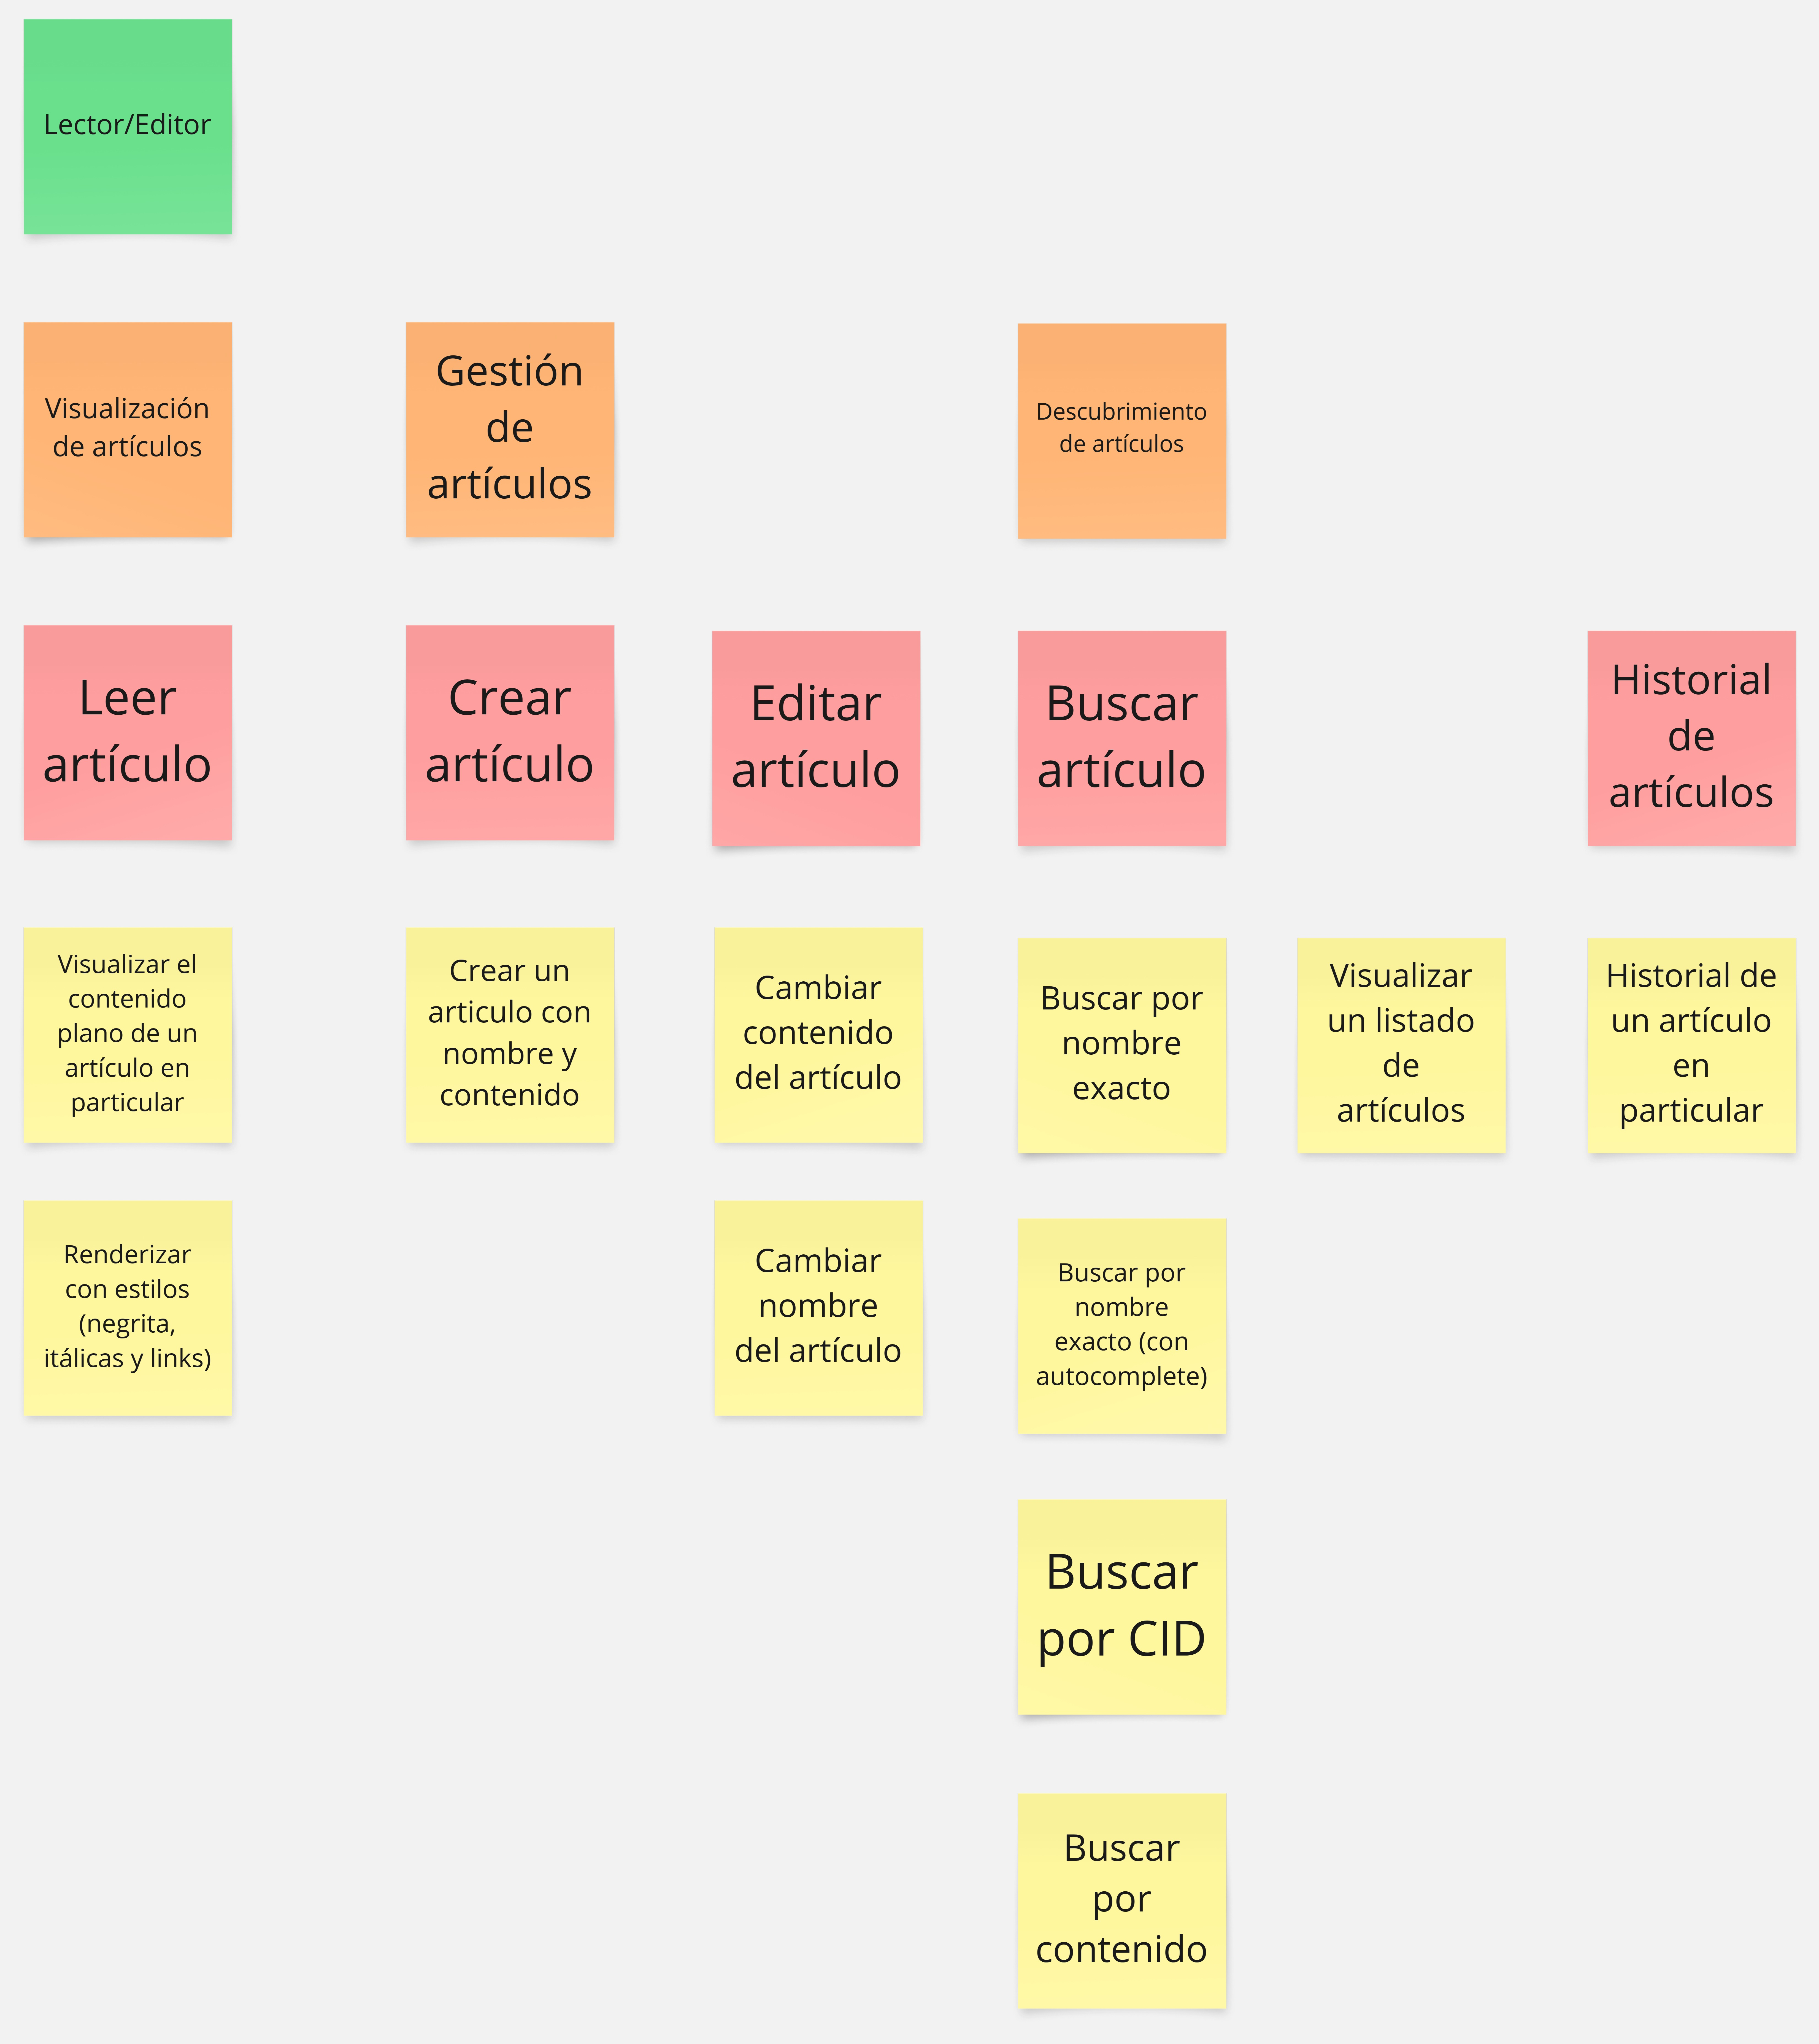
\includegraphics[width=0.5\linewidth]{img/solucion-wiki/usm-wiki.jpg}
    \caption{\textit{User Story Map} del repositorio de conocimiento}
    \label{fig:usm-wiki}
\end{figure}

\subparagraph{Package}

Este caso de uso se implementó en los packages \textbf{Astrawiki} \cite{astrawiki-ipfs} (implementación sobre el ecosistema IPFS) y \textbf{Astrawiki-eth} \cite{astrawiki-eth} (implementación sobre el ecosistema Blockchain). En las subsiguientes secciones, las menciones a Astrawiki referirán a este caso de uso.

\subsubsection{Mensajero en tiempo real}

Este caso se enfoca en la capacidad de la infraestructura de enfrentarse a situaciones de \textit{tiempo real} como puede ser un chat de texto o de audio. En particular, nos centramos en el caso de chats de texto para un grupo de usuarios en donde los mensajes sean públicos.

\paragraph{Requisitos funcionales}

\begin{itemize}
    \item \textbf{Usuarios:} se deben contar con usuarios que puedan iniciar sesión con una clave.
    \item \textbf{Grupos públicos:} grupos de chat de texto, donde cualquier usuario puede ingresar y ver los mensajes del resto, así como también participar enviando sus propios mensajes.
    \item \textbf{Respuestas:} un usuario debe poder responder mensajes anteriores dentro de un mismo chat.
\end{itemize}

\begin{figure}[H]
    \centering
    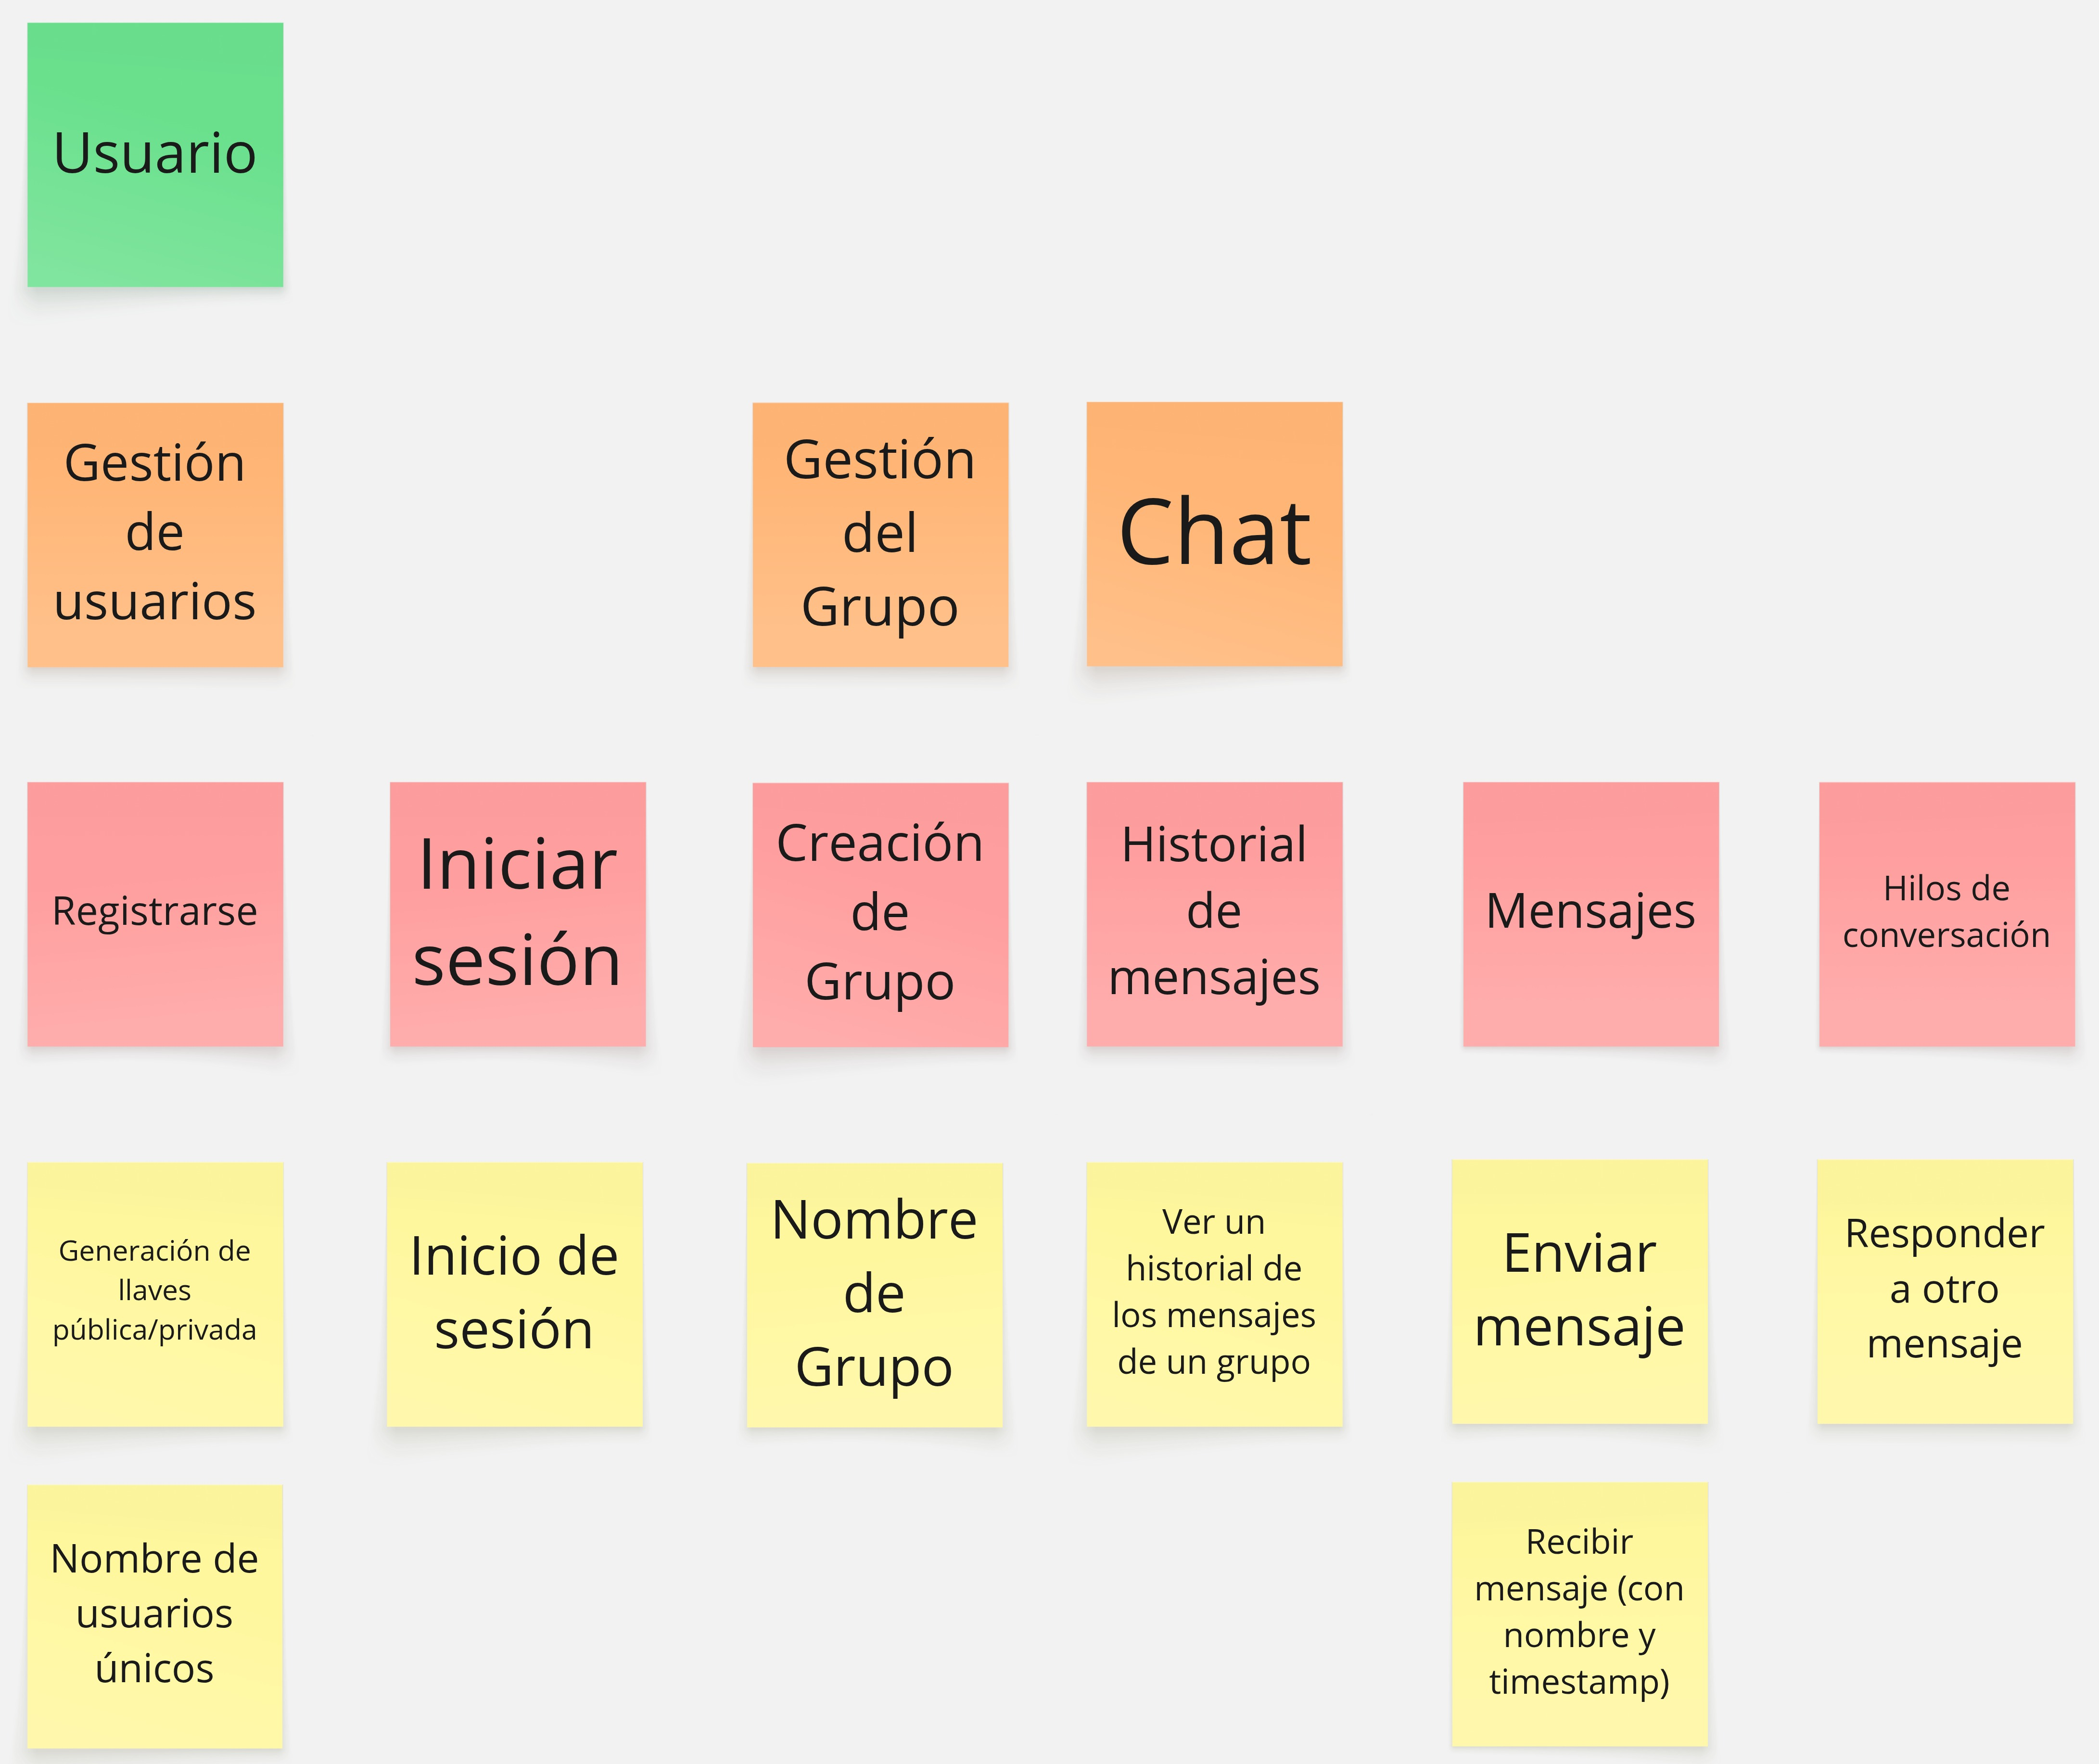
\includegraphics[width=0.5\linewidth]{img/usm-mensajero.jpg}
    \caption{\textit{User Story Map} del mensajero en tiempo real}
    \label{fig:enter-label}
\end{figure}

\subparagraph{Package}

Este caso de uso se implementó en los \textit{packages} \textbf{Astrachat} \cite{astrachat-ipfs} (implementación sobre el ecosistema IPFS) y \textbf{Astrachat-eth} \cite{astrachat-eth} (implementación sobre el ecosistema Blockchain). En las subsiguientes secciones, las menciones a Astrachat referirán a este caso de uso.

\subsection{IPFS}

Durante el desarrollo de los casos de uso sobre el ecosistema IPFS, se fue consolidando una comprensión más profunda de los componentes necesarios para construir aplicaciones distribuidas y descentralizadas. Esto permitió identificar y diseñar una serie de abstracciones que encapsulan la infraestructura general requerida, facilitando la implementación de los casos de uso sobre una base común.

Se distinguen dos infraestructuras principales en funcionamiento: la infraestructura de despliegue y la infraestructura de aplicación.

La \textbf{infraestructura de despliegue} se encarga del alojamiento de las aplicaciones web. Es responsable de distribuir el \textit{front-end} de las aplicaciones, así como también el código necesario para su ejecución, en caso de que incluyan componentes dinámicos. Toda aplicación que deba ser accesible desde la web hace uso de esta infraestructura, como ocurre con el sitio web estático.

Por otro lado, la \textbf{infraestructura de aplicación} gestiona la lógica de la aplicación, incluyendo el almacenamiento de datos y la conexión entre pares. Esta infraestructura es fundamental para aplicaciones que requieren mantener un estado compartido entre usuarios y permitir su modificación, como en el caso del repositorio de conocimiento y el mensajero en tiempo real.

La identificación de estas abstracciones permitió encapsular gran parte de la complejidad asociada al ecosistema subyacente, lo que facilitó el desarrollo tanto de los casos de uso implementados como de posibles desarrollos futuros. Gracias a esta separación, es posible concentrarse exclusivamente en los requisitos funcionales de cada nuevo caso de uso, sin necesidad de interactuar directamente con los detalles técnicos de IPFS y sus herramientas subyacentes.

A continuación, se detalla la composición y el funcionamiento de ambas infraestructuras.

\subsubsection{Infraestructura de despliegue}

El objetivo de la infraestructura de despliegue fue alojar los archivos estáticos de un sitio web en IPFS, y acceder a ellos mediante un navegador, manteniendo su correcta interpretación por el navegador. Además, se priorizó una filosofía de aplicaciones estrictamente comunitarias a la hora de elegir tecnologías y herramientas del ecosistema a utilizar.

Para empezar, se debe explicar brevemente el concepto de \textit{pinning}. Al subir un archivo a IPFS, este se procesa mediante una función de hash, y así se obtiene un \textit{Content Identifier} (CID) único. Desde ese momento, cualquier nodo que desee obtener el archivo puede encontrarlo utilizando dicho CID. Sin embargo, no se asegura la persistencia del archivo, y dejará de ser accesible luego de un tiempo. Por esta razón existe el concepto de \textit{pinning} \cite{pinning}, que consiste en fijar un archivo o directorio para tratar dicha información como esencial y, por lo tanto, evitar que el nodo lo descarte eventualmente. Este concepto es central para la solución implementada.

A continuación se describen brevemente las herramientas utilizadas.

\paragraph{Clústeres colaborativos en IPFS} Un \textit{clúster} es un grupo de nodos de IPFS que actúan en conjunto para fijar contenidos. Funcionan sincronizando su \textit{pin set}, o sea, su lista de archivos y directorios fijados en un momento dado. Un clúster \textit{colaborativo} sigue esta premisa, pero permite que los usuarios colaboren con su nodo local sin posibilidad de modificar los archivos, lo cuál se delega a nodos especiales con la capacidad de orquestar el clúster en conjunto. Así, se logra que la misma comunidad mantenga operativo el mecanismo de despliegue de la aplicación, en línea con la filosofía de aplicaciones comunitarias.

% Actualmente, esta alternativa es poco explorada, por lo tanto no existe una forma fácil de creación, seguimiento y descubrimiento de estos clústeres. IPFS cuenta con una página con clústeres conocidos con los cuales se puede colaborar \cite{collaborative-clusters}, pero la cantidad es limitada.

% Por otro lado, el principal problema es que los clústeres obligan a los nodos a fijar la totalidad de sus archivos, lo cuál puede significar un uso excesivo de almacenamiento necesario para colaborar. Hacer \textit{sharding} sobre el pin set, o sea, fijar parte del contenido de un clúster, es posible utilizando los parámetros de \texttt{replicator\_min} y \texttt{replicator\_max} al agregar un pin, que fijan un límite mínimo y máximo sobre la cantidad de nodos que tienen ese pin. Sin embargo, no es recomendado para clústeres colaborativos debido a la falta de \textit{proof of storage} \cite{cluster-sharding} \cite{collaborative-clusters-setup}. Esto se debe a que, debido a la manera en la que fue diseñada la arquitectura de IPFS, un nodo no confiable puede falsificar la lista de archivos que está fijando, por lo que hay una posibilidad de que una parte del contenido no esté en ninguno de los nodos, y por ende el contenido esté incompleto.

\paragraph{IPNS} El CID cambiará si el contenido del sitio web o aplicación web cambia. Este problema puede ser resuelto con la ayuda de \textit{punteros mutables}, objetos de IPFS que apuntan a un CID específico y pueden ser modificados. Esto permite compartir la dirección del puntero una única vez y actualizar el CID al que apunta cada vez que se haga un cambio. InterPlanetary Name System (IPNS) \cite{ipns} es un sistema que permite crear  punteros mutables y obtener una dirección conocida como \textit{nombre de IPNS}. Estos nombres de IPNS pueden considerarse como enlaces que pueden actualizarse, conservando al mismo tiempo la verificabilidad del content addressing. El titular de la clave privada puede firmar y publicar nuevos registros en cualquier momento.

Una vez que se aloja un contenido en IPFS y se apunta a él mediante un \textit{nombre} de IPNS, el mayor problema pasa a ser la manera de acceder a IPNS en sí. El hecho de que los nombres sean hashes alfanuméricos, y no nombres legibles o memorables para humanos, dificulta el acceso de los usuarios a un sitio web memorable y fácil de compartir. A continuación se analizará la alternativa elegida para solucionar este problema.

\begin{figure}[h]
\centering
\fbox{\texttt{/ipns/k51qzi5uqu5dhkdbjdsauuyk5iyq82uzpjb0is3x6oy9dcmmr8dbcezv7v9fya}}
\caption{Ejemplo de la dirección de un nombre de IPNS}
\end{figure}

Dado que el valor al que apunta el nombre de IPNS cambia con cada modificación del proyecto, se vuelve necesario seleccionar un grupo de nodos que se les confíe con tal fin. De lo contrario un posible atacante podría modificar el registro, invalidándolo o redirigiéndolo. Por la misma razón, no cualquier nodo dentro del clúster debe ser capaz de cambiar el \textit{pin set}, o lista de CIDs fijados por el clúster.

IPFS Cluster tiene en cuenta esto, y hace la distinción entre un nodo \textit{trusted} y un nodo \textit{follower} para su implementación de clústeres \textit{colaborativos} \cite{ipfs-cluster-collaborative}. Para esta herramienta, se utiliza las denominaciones de nodo confiable y nodo colaborador, respectivamente.

\subparagraph{Nodo confiable} Este nodo tiene la capacidad de modificar el nombre IPNS, como también actualizar la configuración del mismo, y el \textit{pin set}. Son una parte esencial del clúster, ya que ellos no es posible modificar el contenido. Esto no implica centralización, ya la comunidad pueden formar sus propios grupos de nodos confiables y actualizar el contenido por su cuenta, similar a realizar un \textit{fork} en un proyecto de Github.

\subparagraph{Nodo colaborador} Únicamente se encarga de fijar los archivos establecidos por los nodos confiables, y actualizar su \textit{pin set} cuando se lo indique. Al igual que los nodos confiables, debe fijar la totalidad de los archivos. Su finalidad es aumentar la disponibilidad del contenido y evitar que la información se pierda.

En un escenario ideal, existen varios nodos confiables disponibles en simultáneo. Esto previene un posible \textit{single point of failure}, y asegura la continuidad y validez del clúster.

\paragraph{ENS} \textbf{Ethereum Name Service (ENS)} \cite{ens} es un protocolo de nombres descentralizado que se basa en la blockchain \textit{Ethereum}. Funciona de manera similar a DNS, en el sentido de que traduce identificadores como nombres y hases a formatos legibles para humanos. Al operar sobre la blockchain de Ethereum, es seguro, descentralizado y transparente. Está diseñado específicamente para traducir identificadores como direcciones de billeteras, hashes y metadatos, entre otros, incluyendo direcciones de IPFS. Es posible configurar un registro ENS que resuelva automáticamente una dirección IPNS. Esto permite usar nombres legibles, más fáciles de compartir y acceder, y soluciona el principal problema de IPNS hasta este punto. Además, cuando se quiera actualizar el contenido, no será necesario modificar el registro ENS en sí, ya que el registro siempre apuntará al mismo nombre de IPNS.

\paragraph{Gateways} Los navegadores modernos no siempre soportan IPFS o ENS de forma nativa. Algunos, como Opera \cite{opera-ipfs} o Brave \cite{brave-ipfs}, permiten acceder directamente a direcciones IPFS o dominios .eth. Sin embargo, la mayoría no ofrece esta funcionalidad, lo que limita el acceso a contenido descentralizado.

Para superar esta limitación, se emplean gateways de Ethereum e IPFS. Un gateway de Ethereum traduce un dominio .eth a una dirección IPNS, mientras que un gateway de IPFS recupera el contenido asociado desde la red distribuida a través de solicitudes HTTP. Algunas gateways tienen la funcionalidad de mostrar una página web de manera correcta cuando un directorio tiene la estructura indicada. Esto resulta particularmente útil para poder mostrar una página moderna de la misma manera que se haría utilizando un servidor HTTP.

\begin{figure}[H]
    \centering
    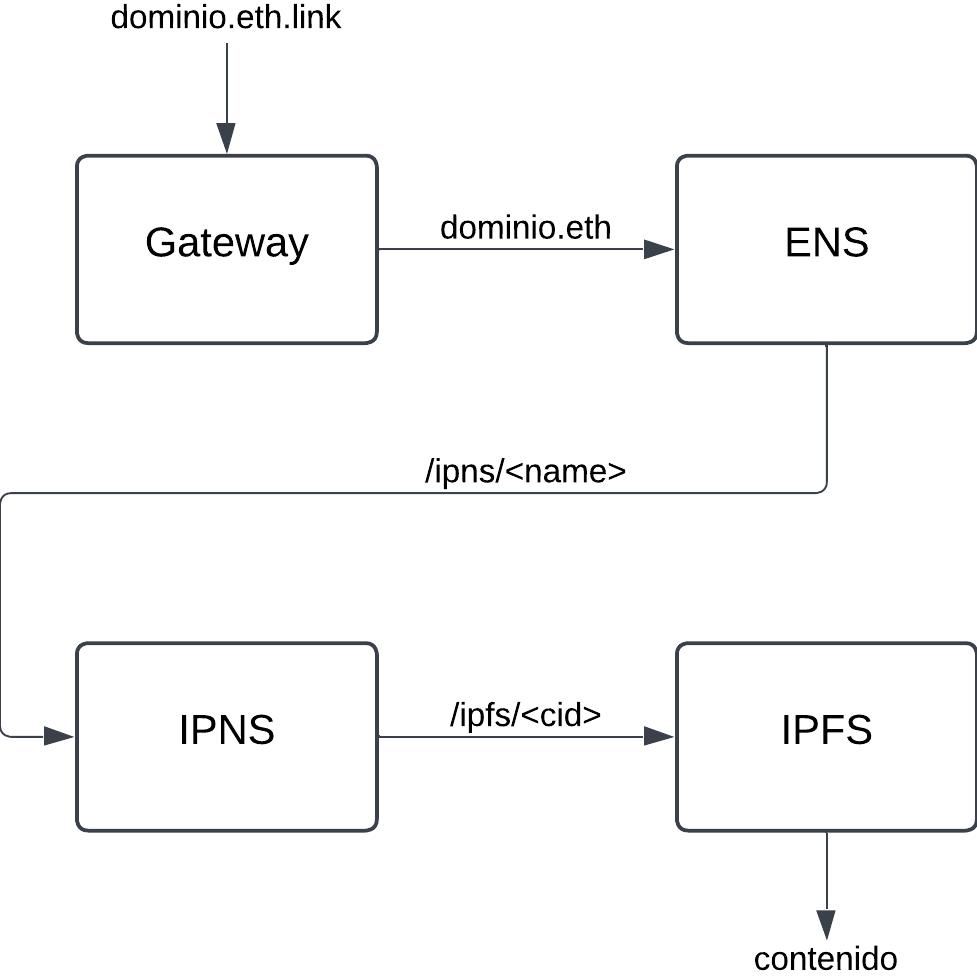
\includegraphics[width=0.5\linewidth]{img/solucion-ipfs/traduccion-dominio.png}
    \caption{Mapa de la traducción de un dominio al contenido de IPFS}
    \label{fig:traduccion-ipfs}
\end{figure}

Para nuestro caso, se utilizó el servicio de Limo \cite{limo}, que soporta direcciones de ENS, y recupera archivos de IPFS, actuando como gateway para ambos servicios. Para utilizarlo, simplemente se requiere agregar un sufijo \texttt{.link} al nombre de ENS. Por ejemplo, \texttt{dominio.eth} puede accederse a través de \texttt{dominio.eth.link}. A su vez, resuelve \texttt{dominio.eth} a una dirección de IPFS, y por lo tanto obtiene los archivos de esa dirección automáticamente.

Si bien las gateways mejoran la accesibilidad desde navegadores tradicionales, también introducen un grado de centralización. Sin embargo, existen múltiples servicios de gateways, tanto de IPFS como de Ethereum, que se pueden utilizar si una de ellas falla.

\paragraph{Despliegue continuo}

Para lograr un despliegue continuo que integre automáticamente un repositorio Git, se diseñó un script que se ejecuta de forma autónoma en cada nodo del clúster. En esta arquitectura mayormente horizontal, no existe un servidor central que orqueste las actualizaciones. Esto elimina un punto único de falla y favorece la resiliencia del sistema. Por lo tanto, cualquier nodo confiable debe poder actualizar su contenido e instruir a los nodos colaboradores para que actualicen su contenido de manera equivalente. Además, el sistema debe funcionar correctamente incluso si los nodos no reciben las actualizaciones simultáneamente, evitando así \textit{race conditions}), es decir, situaciones donde varios procesos intentan modificar un recurso al mismo tiempo.

Como se mencionó anteriormente, debido a la naturaleza del direccionamiento basado en contenido de IPFS, si dos nodos suben el mismo contenido, obtendrán el mismo Content Identifier (CID). Esta propiedad permite que cualquier nodo confiable actualice el contenido y el nombre de IPNS de forma independiente a los demás nodos confiables. Cuando un nodo detecta un cambio nuevo, obtiene el código estático actualizado y, acto seguido, indica a los nodos colaboradores que fijen el CID correspondiente. Si el nodo es el primero en detectar dicha actualización, también instruye al resto del clúster para que dejen de fijar el CID antiguo.

\paragraph{Compilado} Las herramientas de compilación no siempre generan archivos idénticos en compilaciones sucesivas a partir del mismo código fuente, debido a factores como la inclusión de marcas temporales o hashes internos. Por ejemplo, \texttt{Next.js} produce archivos estáticos diferentes incluso cuando el código fuente no cambia, lo cual representa un problema para el enfoque propuesto, ya que dos nodos que compilen localmente el mismo código podrían obtener CIDs distintos y, por ende, no sincronizar correctamente el contenido.

Para mitigar esta situación, se implementó un \textit{hook} automatizado, integrado en el flujo de trabajo del repositorio, que compila el código una única vez por cada \textit{commit} en la rama principal. De este modo, los nodos confiables pueden detectar los cambios en la rama que contiene los archivos compilados, realizar un \textit{pull} de esos archivos ya generados y garantizar que todos obtengan el mismo CID.

\paragraph{Configuración} Para que un usuario pueda conectarse y contribuir como nodo colaborador a un clúster, necesita acceder a una dirección de IPFS desde la cual obtener el archivo \texttt{service.json} \cite{service-json}. Este archivo de configuración contiene la información necesaria para integrarse correctamente al clúster, incluyendo las \textit{multiaddresses} \cite{multiaddr} de los nodos confiables.
Dado que estos nodos pueden agregarse o eliminarse, el archivo está sujeto a modificaciones, por lo que debe ser tratado como parte integral del proceso de despliegue. Cada vez que se actualiza el archivo —por ejemplo, tras un cambio en el repositorio Git donde se aloja—, se debe fijar nuevamente en el clúster y actualizar el nombre de IPNS asociado. De esta forma, los usuarios siempre podrán acceder a la versión actualizada del archivo de configuración mediante un enlace distribuible y verificable.

\begin{figure}[H]
\centering
\fbox{\texttt{/ip4/123.123.123.123/udp/9096/quic/p2p/12D3KooWLw...yPcuZJR}}
\caption{Ejemplo de una \textit{multiadress} posible que utiliza el protocolo QUIC.}
\end{figure}

\paragraph{Limitaciones}

Este enfoque, si bien permite un despliegue descentralizado y gestionado por la comunidad, presenta algunas limitaciones técnicas y operativas:

\subparagraph{Actualización completa del contenido} Cada vez que se realice un cambio en el directorio de la aplicación, se deberá fijar una nueva versión completa del contenido. Esto obliga a los nodos colaboradores a descargar nuevamente todo el directorio, lo que puede implicar un costo elevado en términos de ancho de banda y tiempo, especialmente para archivos de gran tamaño.

\subparagraph{Problemas de cacheo en IPNS} El parámetro TTL de IPNS determina cuánto tiempo permanece un valor en la caché de un nodo antes de consultarse nuevamente en la DHT. Si se configura un TTL alto, los cambios recientes pueden demorar en propagarse. En cambio, un TTL bajo reduce la latencia de actualización pero incrementa el número de consultas a la red, lo cual puede afectar el rendimiento. No obstante, cada nodo mantiene siempre la última versión del nombre que haya resuelto correctamente.

\subparagraph{Distribución de claves privadas} Como las actualizaciones de IPNS requieren estar firmadas con una clave privada, todos los nodos confiables deben compartir la misma clave para poder emitir registros válidos. Esto elimina el punto único de falla, pero al mismo tiempo incrementa el riesgo de exposición si la clave es comprometida.

\subparagraph{Requerimiento de apertura de puertos} La operación de IPFS Cluster exige la apertura del puerto 9096 para la comunicación entre nodos. Este requerimiento puede representar una barrera para ciertos usuarios, especialmente aquellos con configuraciones de red restrictivas o sin conocimientos técnicos avanzados.

\paragraph{Implementación del nodo confiable}

En base a este análisis, podemos concluir que la mejor forma de desplegar una página web estática en IPFS es a través del uso de un clúster colaborativo compuesto por nodos confiables que se integren con el proyecto de Git dado, así como una dirección IPNS a la cuál actualizar cada vez que hay un cambio, y un registro ENS para traducir la dirección IPNS a un nombre legible.

\subparagraph{Arquitectura general}

La herramienta está compuesta por tres contenedores:
\begin{itemize}
    \item \textbf{Kubo:} el nodo de IPFS encargado de conectarse a la red de IPFS para publicar y obtener el contenido necesario.
    \item \textbf{IPFS Cluster:} gestiona el contenido fijado y coordina con otros nodos del clúster.
    \item \textbf{Watcher:} observa los repositorios de Git del proyecto y del archivo \texttt{service.json}, y orquesta acciones en los otros dos contenedores.
\end{itemize}

La comunicación entre contenedores se realiza a través de sus respectivas APIs HTTP \cite{kubo-api} \cite{cluster-api}. El contenedor watcher está basado en Alpine Linux y utiliza scripts POSIX-compliant para máxima portabilidad.

\begin{figure}[H]
    \centering
    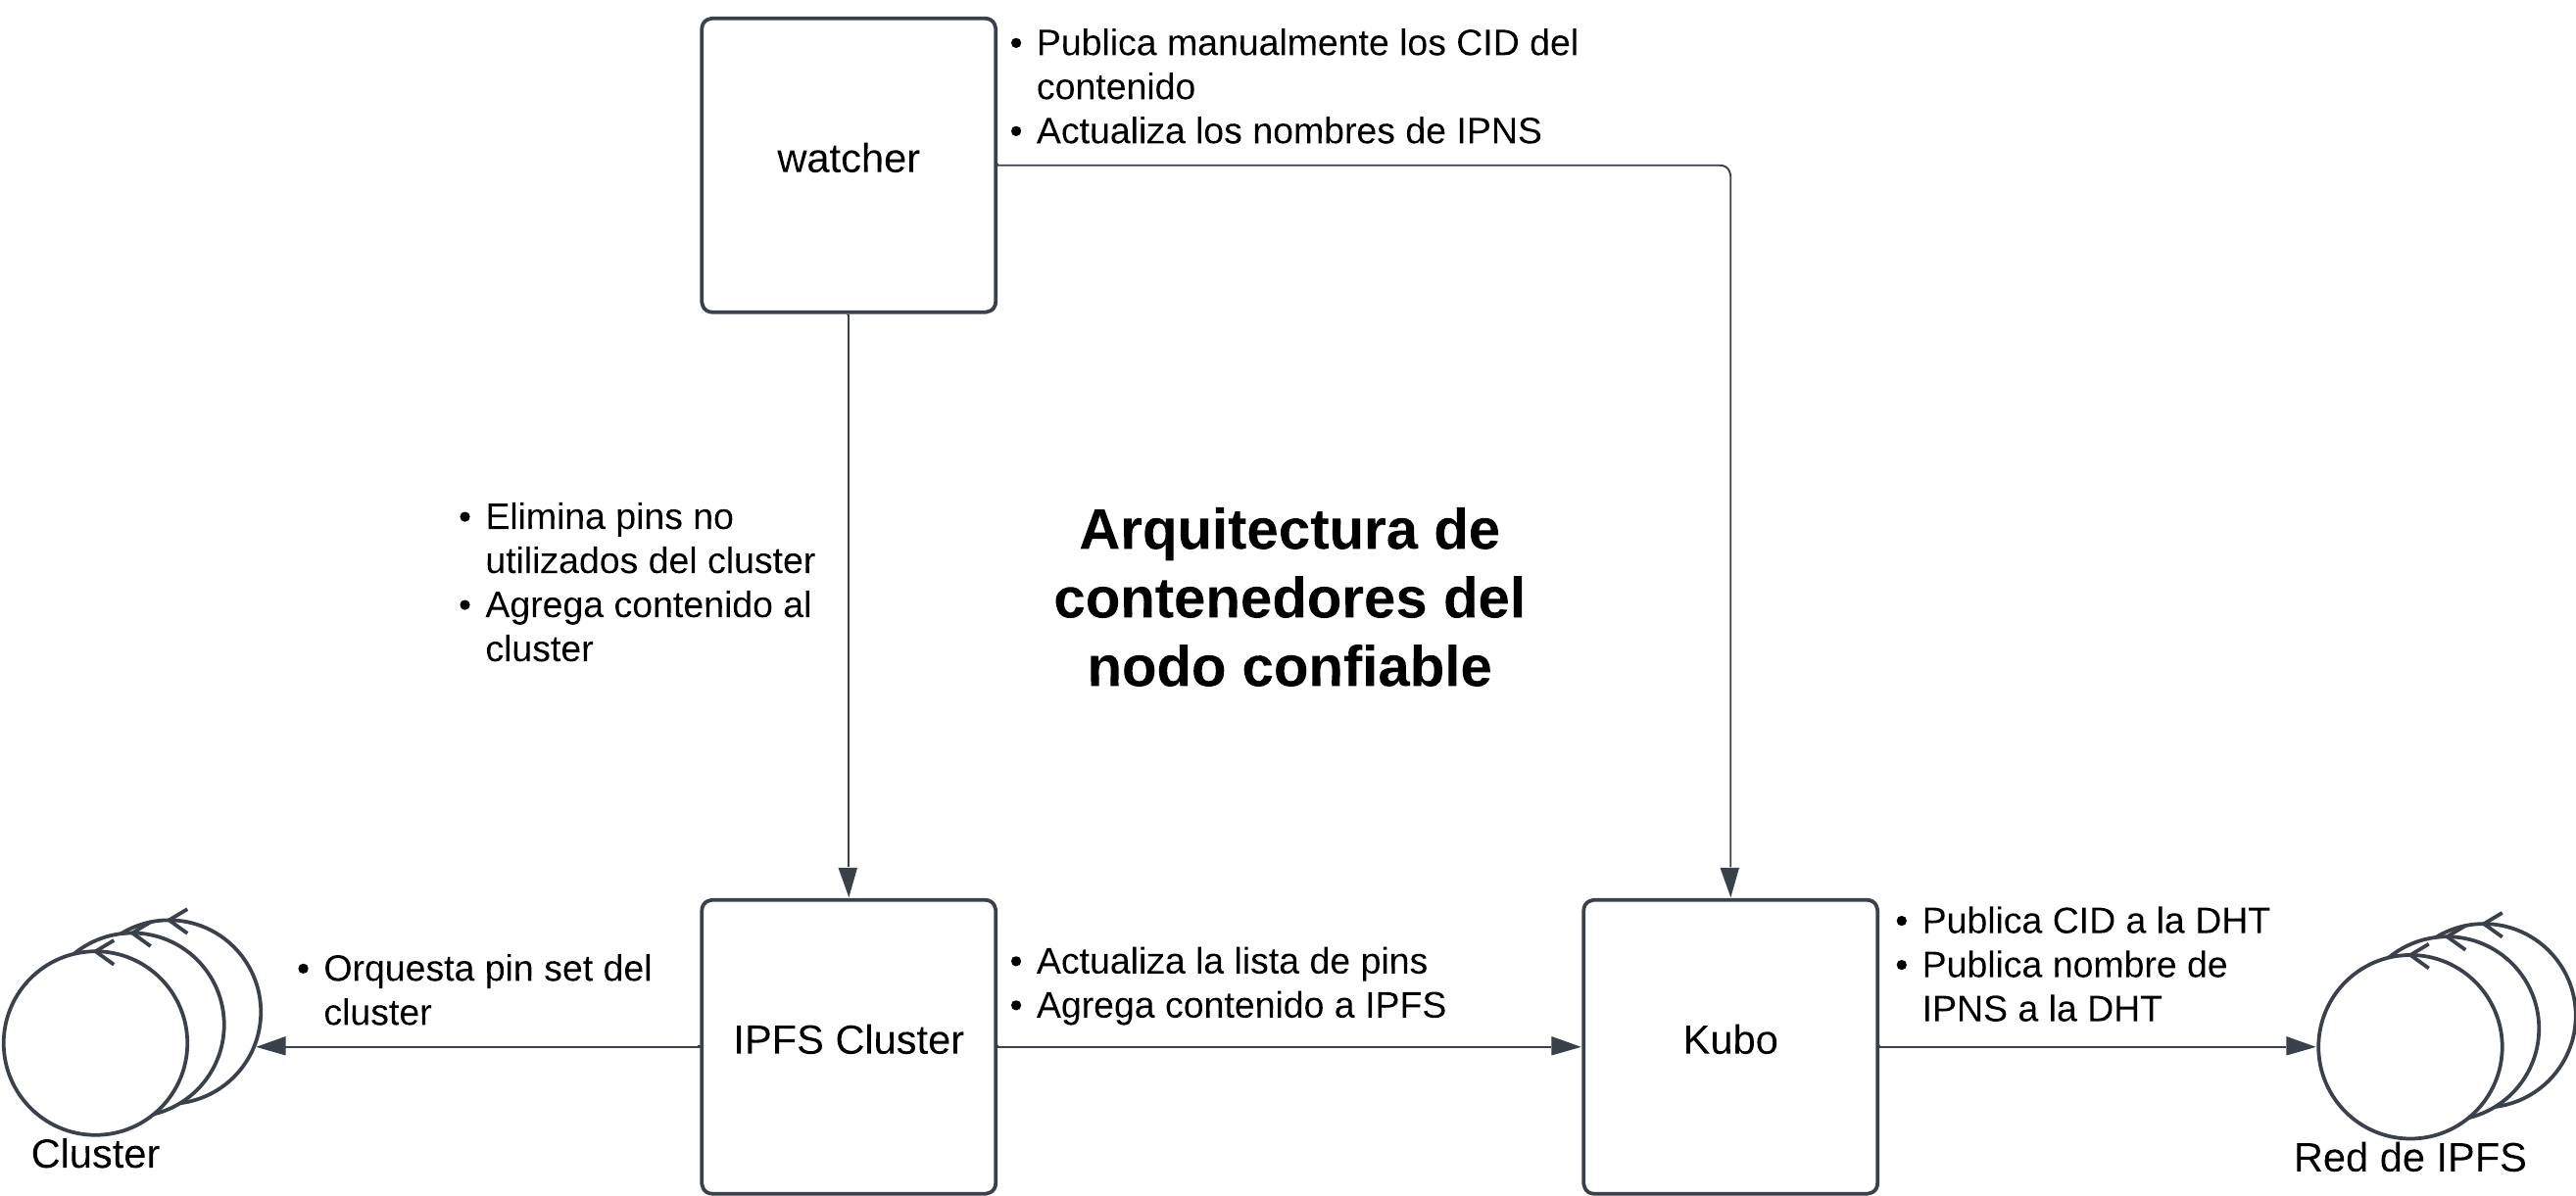
\includegraphics[width=1\linewidth]{img/solucion-ipfs/contenedores-trusted-peer.png}
    \caption{Mapa de interacciones entre los contenedores del nodo confiable}
    \label{fig:contenedores-trusted-peer}
\end{figure}

\subparagraph{Pipeline de despliegue} El contenedor watcher compara periódicamente el último commit de una rama remota con una copia local clonada al iniciar. Al detectar un cambio en el contenido o en el archivo \texttt{service.json}, ejecuta el siguiente flujo:
\begin{enumerate}
    \item Sube el contenido y el archivo \texttt{service.json} al clúster, obteniendo sus respectivos CIDs.
    \item Publica manualmente ambos CIDs en la red IPFS usando Kubo.
    \item Verifica que todos los nodos del clúster hayan fijado los nuevos CIDs.
    \item Actualiza los registros IPNS correspondientes.
    \item Elimina los pins antiguos del clúster para liberar recursos.
\end{enumerate}

\begin{figure}[H]
    \centering
    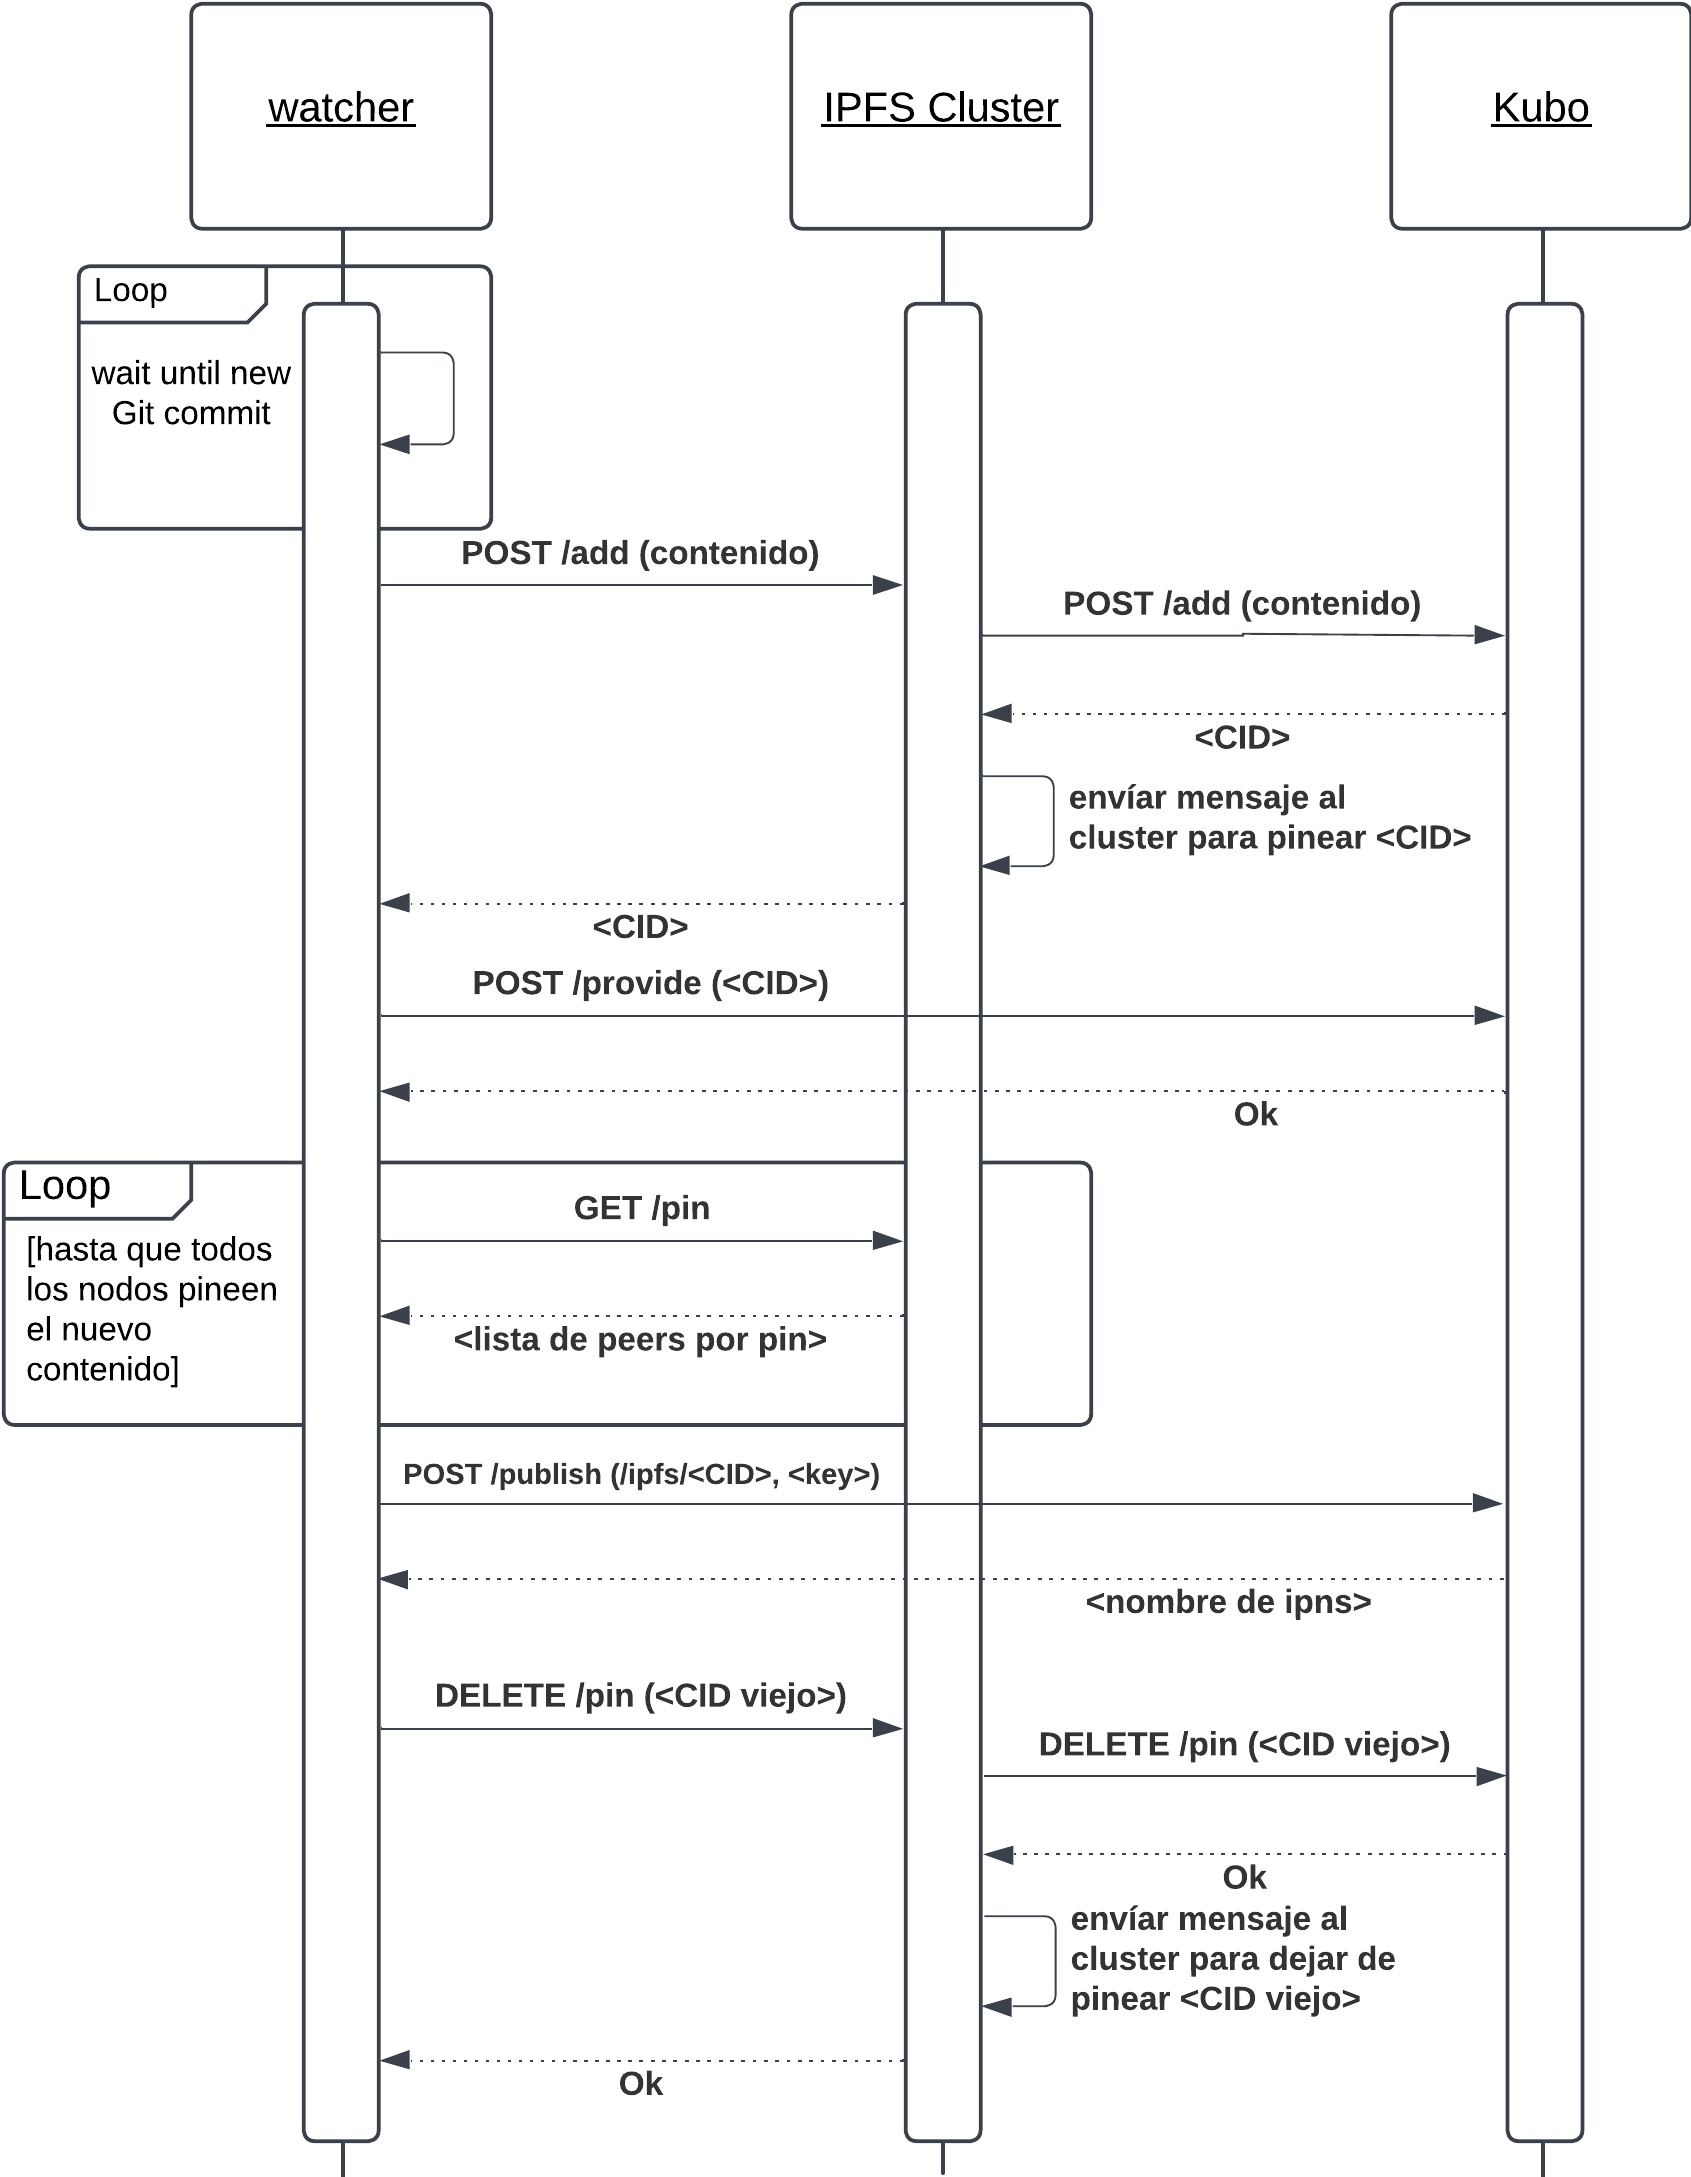
\includegraphics[width=0.5\linewidth]{img/solucion-ipfs/ds-trusted-peer.png}
    \caption{Diagrama de secuencia para el caso en que watcher detecta un cambio. Notar que para mayor claridad se omite los pasos para desplegar el nombre de IPNS del \texttt{service.json}, al ser exactamente los mismos que en el caso de un contenido.}
    \label{fig:ds-contenedores-trusted-peer}
\end{figure}

\subparagraph{Gestión de claves de IPNS}

Cada nodo confiable requiere una identidad persistente, definida por un PeerID y su clave privada, que debe conservarse entre ejecuciones. Esta identidad es la que figura en el archivo \texttt{service.json}, el cual los nodos colaboradores utilizan para unirse al clúster.

Además, todos los nodos confiables deben compartir las mismas claves privadas de IPNS para poder actualizar los registros. Se utilizan dos claves distintas: una para el contenido estático y otra para \texttt{service.json}. Un script interactivo facilita la generación inicial de estas configuraciones, incluyendo identidad, claves IPNS, direcciones de repositorios y demás parámetros necesarios.

\subparagraph{Disponibilidad} Dos factores pueden afectar la disponibilidad del contenido:

\begin{itemize}
    \item \textbf{Propagación del IPNS:} Un nuevo valor puede no estar aún distribuido en toda la DHT. Por ello, se garantiza primero la publicación exitosa del nuevo valor antes de eliminar el contenido anterior del clúster.
    \item \textbf{Indexación del nuevo CID:} Publicar el contenido manualmente mediante Kubo antes de actualizar el IPNS asegura que esté accesible de forma inmediata desde gateways o nodos externos.
\end{itemize}

Este enfoque añade una latencia al proceso de actualización, pero asegura la disponibilidad continua de al menos una versión válida del contenido.

% \subparagraph{Integración con Git}

% La manera en la que el contenedor \textit{watcher} puede detectar un cambio en el repositorio es consultando el repositorio remoto de Git cada minuto para identificar un cambio realizado y accionar el script de despliegue. Se requiere que el repositorio del contenido sea público, ya que la identificación por SSH o usuario y clave no están disponibles fácilmente dentro de un contenedor. De todas maneras, el contenido o archivos estáticos en el caso de una aplicación web ya son públicos por naturaleza, y debido al enfoque comunitario dado, que un repositorio necesite ser público no representa una restricción apreciable.

\subparagraph{Resultado}

La solución permite instanciar un nodo confiable mediante un único comando (\texttt{make up}), el cual se encarga automáticamente del monitoreo, despliegue y publicación del contenido en IPFS. Aunque está optimizada para aplicaciones web, la herramienta es agnóstica respecto al tipo de contenido, siendo apta también para documentación, recursos estáticos o repositorios.

Combinada con un registro ENS y un gateway compatible, esta solución ofrece una experiencia de usuario comparable a la de un servidor HTTP moderno, pero con las ventajas inherentes de una infraestructura comunitaria, descentralizada y de bajo costo.

\subsubsection{Infraestructura de aplicación}

Las aplicaciones dinámicas, aquellas que requieren mantener un estado mutable, como un repositorio de conocimiento o un mensajero en tiempo real, presentan desafíos particulares en el ecosistema de IPFS. Si bien IPFS permite mantener un estado compartido mediante la publicación continua de nuevos CIDs y el uso de mecanismos como IPNS —el cual introdujimos y utilizamos en la infraestructura de despliegue—, \textbf{no está diseñado específicamente para la actualización eficiente de datos dinámicos en tiempo real}.

Esto introduce ciertas limitaciones a la hora de construir aplicaciones interactivas, donde múltiples usuarios necesitan leer y escribir datos de forma concurrente. En particular, la falta de mecanismos nativos para gestionar versiones, sincronizar cambios o evitar conflictos entre ediciones simultáneas hace que desarrollar aplicaciones con estado mutable directamente sobre IPFS resulte poco conveniente.

Para superar estas limitaciones, desarrollamos \textbf{AstraDB}, una infraestructura pensada para facilitar la creación y gestión de aplicaciones dinámicas y colaborativas dentro del ecosistema de IPFS.

A continuación, describiremos los componentes y la arquitectura de \textbf{AstraDB}, cómo permite representar entidades como artículos o conversaciones, y cómo se adapta a las necesidades de aplicaciones comunitarias y descentralizadas, tales como wikis colaborativas y sistemas de mensajería en tiempo real.

\paragraph{AstraDB}

AstraDB es una infraestructura diseñada para facilitar el desarrollo de aplicaciones comunitarias, distribuidas y descentralizadas que requieren mantener un estado mutable. Construida como una capa superior a \textbf{OrbitDB} \cite{orbitdb}, abstrae muchos de los aspectos de bajo nivel necesarios para operar bases de datos en redes peer-to-peer.

Su diseño prioriza la colaboración entre múltiples usuarios, permitiendo que cualquier persona pueda contribuir activamente al sostenimiento de la aplicación sin depender de servidores centrales ni infraestructura dedicada. Para ello, automatiza tareas fundamentales como la sincronización, el descubrimiento de nodos y la replicación de datos entre colaboradores.

AstraDB expone una interfaz simple inspirada en el modelo de pares \textit{clave-valor}, donde cada entidad —como una conversación o un artículo— se asocia a una clave única. Las operaciones principales permiten agregar nuevos valores bajo una clave, consultar los valores existentes y suscribirse a actualizaciones en tiempo real, facilitando así el desarrollo de aplicaciones colaborativas sin exponer al desarrollador a la complejidad del entorno distribuido.

\paragraph{Representación de los datos}

AstraDB utiliza OrbitDB para la representación de sus datos. OrbitDB es una base de datos distribuida peer-to-peer que utiliza IPFS para el almacenamiento y \textbf{libp2p} \cite{libp2p} para la sincronización entre nodos. Es una base de datos \textit{eventualmente consistente}, diseñada específicamente para operar en redes descentralizadas sin depender de servidores centrales, lo que la hace especialmente adecuada para aplicaciones distribuidas.

OrbitDB ofrece distintos tipos de bases de datos, adaptadas a diversos modelos y casos de uso, como bases de documentos o estructuras de eventos secuenciales.

Con el objetivo de garantizar una verdadera descentralización y evitar que exista una entidad con permisos privilegiados, AstraDB utiliza bases de datos del tipo de eventos, las cuales son \textit{append-only}. Este tipo de base de datos mantiene un historial inmutable de entradas, donde los nodos pueden únicamente agregar nuevos registros sin posibilidad de modificar o eliminar los existentes. Esto asegura la integridad y preservación de la información, permitiendo que cualquier usuario pueda contribuir sin comprometer la consistencia del sistema.

Esta decisión de trabajar con estructuras \textit{append-only} introduce, sin embargo, un nuevo desafío: ¿cómo representar información actualizable si no se puede sobrescribir el valor de una clave?

La solución adoptada por AstraDB consiste en asignar a cada clave su propia base de datos de eventos. De esta forma, por ejemplo, un artículo puede representarse como una secuencia de actualizaciones almacenadas en orden cronológico. Cada entrada en la base corresponde a un cambio realizado sobre esa entidad, y su historia completa permite reconstruir su versión más reciente o auditar su evolución a lo largo del tiempo.

\begin{figure}[H]
\centering
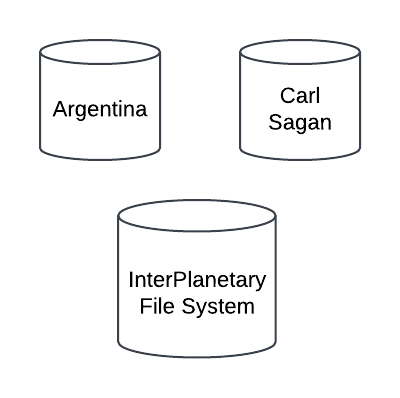
\includegraphics[width=0.4\linewidth]{img/solucion-ipfs/bdd-articulos.png}
\caption{Cada entidad se representa con su propia base de datos de eventos.}
\label{fig:bdd-articulos}
\end{figure}

Este enfoque también permite una distribución eficiente: dado que en OrbitDB cada base de datos debe ser replicada localmente para poder ser leída, AstraDB permite que cada nodo sincronice únicamente las claves (y, por ende, las bases) que le interesan. Esto reduce significativamente la carga de almacenamiento y comunicación.

Para registrar qué claves existen dentro de una instancia de AstraDB —por ejemplo, qué artículos están presentes en un repositorio de conocimiento— se utiliza una base de datos adicional, también del tipo de eventos, que funciona como índice global. Allí se agregan nuevas claves a medida que se crean, permitiendo a los nodos descubrir las entidades disponibles sin necesidad de conocer todo el sistema de antemano.

\begin{figure}[H]
\centering
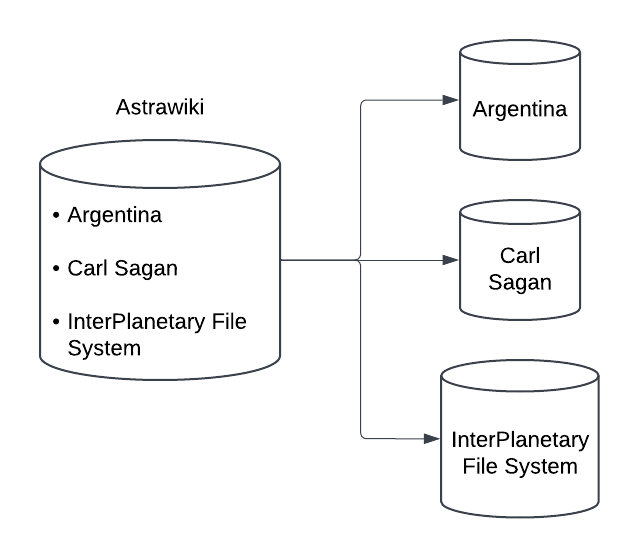
\includegraphics[width=0.6\linewidth]{img/solucion-ipfs/bdd-wiki.png}
\caption{Base de datos de eventos que funciona como índice global de claves.}
\label{fig:bdd-wiki}
\end{figure}

\paragraph{Identificación y acceso a los datos}

Cada base de datos en AstraDB se identifica a través de una dirección única generada por OrbitDB. Esta dirección está compuesta por tres elementos: el tipo de base, su controlador de acceso y un nombre identificador. Dado que AstraDB utiliza siempre el mismo tipo (eventos) y un controlador abierto —que permite a cualquier usuario agregar información—, la dirección final queda determinada únicamente por el nombre elegido.

Esta propiedad resulta fundamental para el funcionamiento del sistema. Permite que cualquier nodo, con solo conocer el nombre de una entidad, pueda acceder a la base de datos y sincronizarse con el resto de los nodos que ya la están replicando. Esto se debe a que crear una base de datos con el mismo nombre no genera una nueva, sino que devuelve la misma dirección y, por lo tanto, accede a la misma base.



\begin{figure}[H]
\centering
\fbox{\texttt{/orbitdb/zdpuAmrcSRUhkQcnRQ6p4bphs7DJWGBkqczSGFYynX6moTcDL}}
\caption{Ejemplo de dirección de una base de datos en OrbitDB.}
\end{figure}

AstraDB extiende este mecanismo de identificación para construir jerarquías lógicas de entidades. Por ejemplo, el nombre de una base puede componerse como \texttt{wiki:articulo}, lo que permite organizar de forma estructurada grandes cantidades de datos.

\begin{figure}[H]
\centering
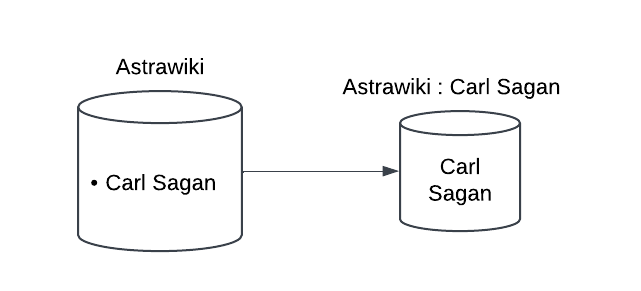
\includegraphics[width=0.6\linewidth]{img/solucion-ipfs/bdd-names.png}
\caption{Estructura jerárquica de claves identificadoras.}
\label{fig:bdd-names}
\end{figure}

Este enfoque también permite que múltiples instancias de AstraDB convivan de forma completamente independientes. La identidad de cada instancia —es decir, el conjunto de claves y sus respectivas bases de valores— queda determinada por el nombre identificador utilizado para crear su base de datos central. De este modo, es trivial crear nuevas aplicaciones, wikis o sistemas colaborativos simplemente utilizando nombres distintos, sin generar colisiones ni interferencias con otras instancias.

\begin{figure}[H]
\centering
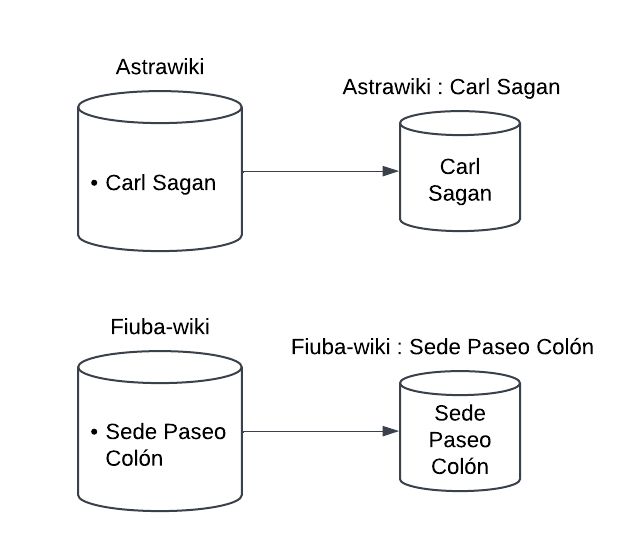
\includegraphics[width=0.6\linewidth]{img/solucion-ipfs/bdd-multiple.png}
\caption{Representación de múltiples instancias independientes de AstraDB.}
\label{fig:bdd-multiple}
\end{figure}

\paragraph{Sincronización y manejo de eventualidad}

En OrbitDB la sincronización entre nodos ocurre de forma eventual, lo que significa que, con el tiempo, todas las instancias de una misma base de datos tenderán a contener la misma información, pero no necesariamente en el mismo orden o al mismo tiempo.

OrbitDB emite eventos cuando una base de datos es actualizada, lo cual resulta crucial para AstraDB, especialmente al sincronizarse con otros nodos y recibir nuevas entradas. Sin embargo, debido a la naturaleza eventual de la consistencia que caracteriza a OrbitDB, y aunque se esté utilizando una base de datos de tipo evento secuencial, la entrada que desencadena el evento de actualización no siempre representa la última inserción cronológica. Es posible que, tras la sincronización, contenido aparezca antes o después de entradas más recientes en la estructura interna de la base de datos.

Para abordar esta situación, AstraDB implementa una capa de abstracción sobre OrbitDB que permite detectar todas las entradas nuevas, independientemente de su posición. Esta abstracción mantiene un registro de los identificadores \textit{hash} de las entradas previamente vistas, y al recibir un evento de actualización, recorre toda la base de datos en busca de nuevas entradas aún no notificadas, emitiendo un evento por cada una de ellas.

Este mecanismo resulta especialmente importante en aplicaciones como el mensajero en tiempo real, donde es necesario garantizar que ningún mensaje pase desapercibido, incluso si fue insertado en una posición intermedia de la base de datos como resultado de la fusión de dos instancias previamente desincronizadas.

\begin{figure}[H]
\centering
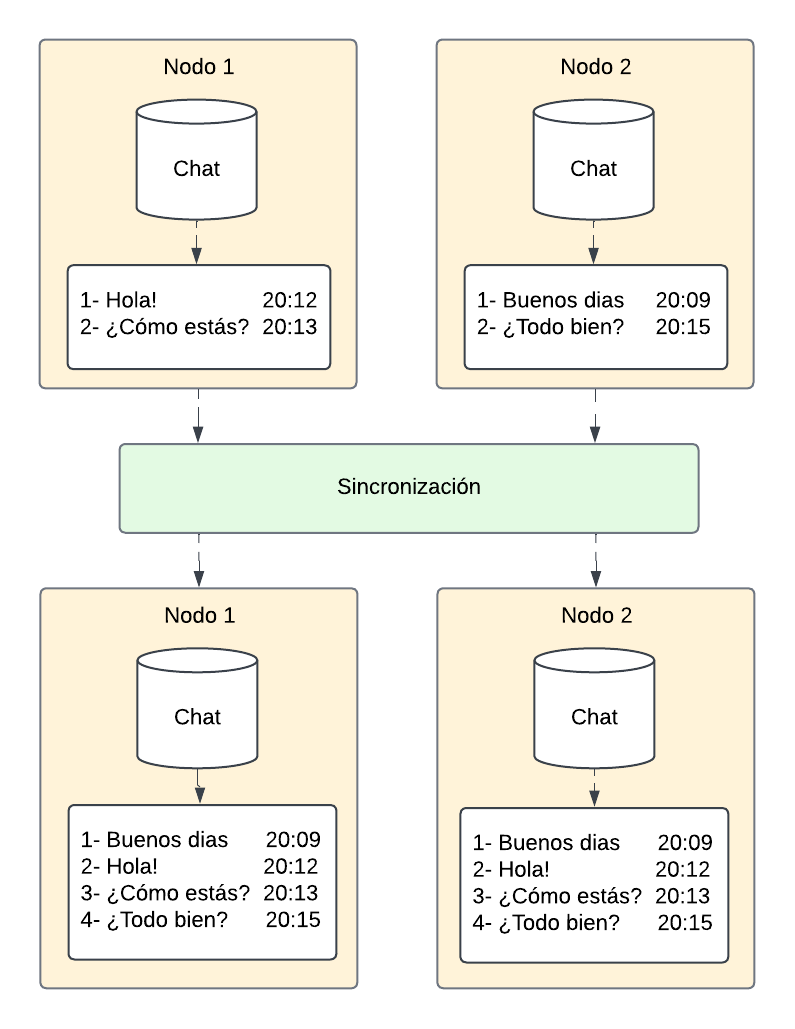
\includegraphics[width=0.7\linewidth]{img/solucion-ipfs/ejemplo-sincronizacion.png}
\caption{Ejemplo de sincronización entre nodos.}
\label{fig:ejemplo-sincronizacion}
\end{figure}

La Figura~\ref{fig:ejemplo-sincronizacion} ilustra este fenómeno: dos nodos mantienen versiones distintas de una misma base de datos denominada ‘Chat’. Tras la sincronización, OrbitDB fusiona ambas versiones, generando una nueva instancia consistente. No obstante, desde la perspectiva del nodo 1, las nuevas entradas pueden no encontrarse exclusivamente al final de la base de datos, y la única notificación automática emitida por OrbitDB corresponde a la última entrada añadida. Por ello, es indispensable recorrer toda la base para garantizar la detección completa de las entradas incorporadas durante la sincronización.

\paragraph{Colaboradores}

En AstraDB, cada instancia existente de base de datos de OrbitDB —al abrirse— debe encontrar a otros nodos que ya la estén replicando para poder sincronizar su contenido. Si no hay ninguno disponible, la base aparece vacía, lo que implica una posible pérdida de información si no hay nodos que la conserven.

Para resolver este problema, AstraDB introduce el concepto de colaboradores: nodos que optan por conservar y replicar activamente todas las bases de datos existentes. En el caso del repositorio de conocimiento, por ejemplo, esto implica mantener localmente cada uno de los artículos publicados en el sistema.

La existencia de al menos un colaborador conectado garantiza que cualquier usuario pueda acceder al contenido completo de una base. De este modo, la red no depende de una infraestructura centralizada, sino de la voluntad de los usuarios de participar activamente en la preservación de la aplicación.

A diferencia de otros enfoques distribuidos basados en incentivos económicos, AstraDB se apoya en un modelo comunitario: cualquier persona puede convertirse en colaborador, sin necesidad de permisos especiales ni recompensas. Su única función es brindar persistencia a las bases que almacena, ayudando a que el sistema permanezca accesible.

\paragraph{Conectividad}

Para que la sincronización entre distintas bases de datos de OrbitDB ocurra, primero deben estar ambos pares conectados. Dada la naturaleza de consistencia eventual con la que trabaja OrbitDB, este no se responsabiliza por el establecimiento ni el mantenimiento de las conexiones entre nodos, simplemente asume que, si dos nodos están conectados, eventualmente sincronizarán sus réplicas.  Por eso, en su lugar, delega completamente esta tarea a la capa subyacente de red, que en este caso está conformada por \textbf{LibP2P} \cite{libp2p}, a través de la implementación provista por \textbf{Helia} \cite{helia}. Esto implica que es nuestra responsabilidad definir cómo se comunican los nodos, seleccionando explícitamente qué protocolos de transporte utilizar según el entorno en el que se ejecutan.

LibP2P es una biblioteca modular diseñada para construir redes peer-to-peer. No define una única forma de conexión, sino que ofrece un conjunto de componentes intercambiables —como transporte, cifrado, multiplexación o descubrimiento de pares— que pueden combinarse según las necesidades del entorno. Esta flexibilidad es clave para nuestra infraestructura, ya que nos permite adaptar el comportamiento de los nodos a las restricciones del entorno web o aprovechar las capacidades completas de un proceso independiente.

LibP2P proporciona distintos protocolos de transporte que permiten que dos nodos mantengan una conexión persistente. Cada nodo puede configurarse con múltiples protocolos, y la elección depende de dónde se ejecuta ese nodo. En nuestra infraestructura, distinguimos entre:

\begin{itemize}
    \item \textbf{Nodos independientes}, que corren en entornos como node.js
    \item \textbf{Nodos web}, que se ejecutan dentro de un navegador.
\end{itemize}

Los nodos independientes utilizan \textbf{TCP} como protocolo principal. Es estable, ampliamente soportado y no presenta restricciones técnicas en entornos controlados. Este protocolo permite que los nodos colaboradores se comuniquen entre sí directamente.

Por otro lado, los nodos web presentan mayores restricciones. Los navegadores modernos no permiten conexiones TCP o UDP directas por razones de seguridad, y limitan las conexiones a protocolos seguros que cumplan con políticas de contexto seguro (\textit{Secure Context}), como HTTPS.

Para resolver esta limitación, la infraestructura utiliza \textbf{WebRTC-Direct}, un protocolo de transporte compatible con navegadores que permite conexiones directas entre un nodo web y un nodo independiente. WebRTC es una tecnología estándar para aplicaciones en tiempo real, como llamadas de video o intercambio de archivos. LibP2P lo adapta para lograr una conexión peer-to-peer entre nodos, sin depender de certificados ni servidores intermediarios.

Gracias a esta combinación de protocolos \textbf{—TCP para nodos independientes y WebRTC-Direct para nodos web—}, se logra una red completamente funcional en la que cualquier nodo puede conectarse con otros, incluso desde el navegador, sin comprometer la descentralización de la arquitectura.

\begin{figure}[H]
\centering
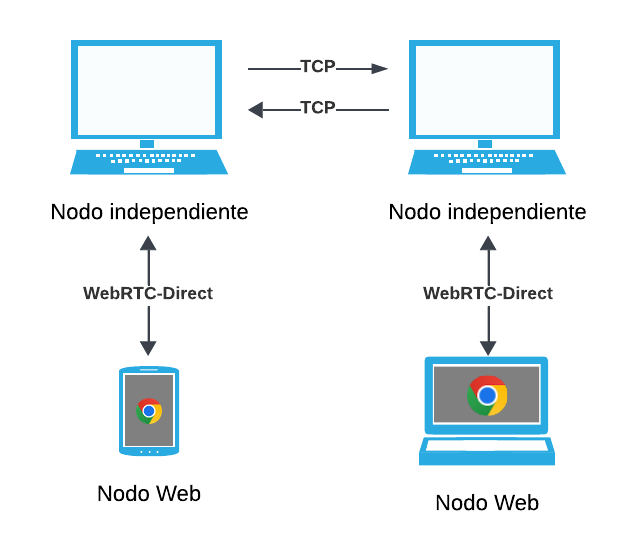
\includegraphics[width=0.55\linewidth]{img/solucion-ipfs/topologia.png}
\caption{Topología de conexiones entre nodos independientes y nodos web.}
\label{fig:topologia-conexiones}
\end{figure}

\paragraph{Descubrimiento de colaboradores}

En la infraestructura de AstraDB, además de definir los protocolos de transporte y la forma en que los nodos se conectan, es fundamental abordar el mecanismo mediante el cual un nodo identifica a qué otros nodos debe conectarse para sincronizar y obtener la base de datos, es decir, cómo se realiza el descubrimiento de colaboradores.

Para preservar la naturaleza descentralizada del sistema, esta función se implementa aprovechando el modelo de descubrimiento de contenido que utiliza IPFS. IPFS se basa en un esquema de \textit{content addressing} \cite{content-addressing}, donde los datos son identificados y accedidos a través de un identificador único basado en su contenido, conocido como Content Identifier (CID), en lugar de su ubicación física.

La localización del contenido en IPFS se efectúa mediante una Distributed Hash Table (DHT), que funciona como una base de datos distribuida. Cada nodo mantiene una porción del índice global que asocia cada CID con los nodos proveedores de dicho contenido. Cuando un nodo desea acceder a un contenido específico, consulta la DHT para identificar los proveedores activos correspondientes \cite{dht}.

Este mecanismo se adopta directamente en AstraDB para el descubrimiento de colaboradores. Al considerar que el CID representa la base de datos —derivada de su nombre identificador— y que los colaboradores son los nodos que proveen ese CID, un nodo interesado realiza una consulta en la DHT para obtener una lista de nodos activos replicando la base. De esta forma, se establece un enfoque completamente descentralizado en el que los colaboradores anuncian su disponibilidad y los nodos nuevos pueden descubrirlos y sincronizarse sin depender de nodos preconfigurados ni puntos centrales.

\paragraph{Identidad de los usuarios}

En AstraDB, los usuarios no se identifican mediante nombres de usuario centralizados, sino a través de un esquema criptográfico basado en claves públicas y privadas, gestionado mediante las identidades de OrbitDB.

Si al iniciar un nodo de AstraDB no se proporciona una clave privada, se genera automáticamente una nueva identidad. La clave privada asociada puede luego ser exportada y almacenada, permitiendo preservar la identidad del nodo entre sesiones.

\paragraph{Arquitectura}

La infraestructura de AstraDB se sustenta en los conceptos y tecnologías detallados en las secciones anteriores, integrando el almacenamiento descentralizado mediante IPFS y OrbitDB, junto con el manejo de conexiones peer-to-peer a través de LibP2P. Esta base técnica permite construir una arquitectura modular que separa claramente el manejo de datos y el manejo de conexiones.

Dicha arquitectura está compuesta por dos componentes principales que operan en paralelo y de manera independiente: el \textit{Key Repository} y el \textit{Connection Manager}.

\begin{figure}[H]
\centering
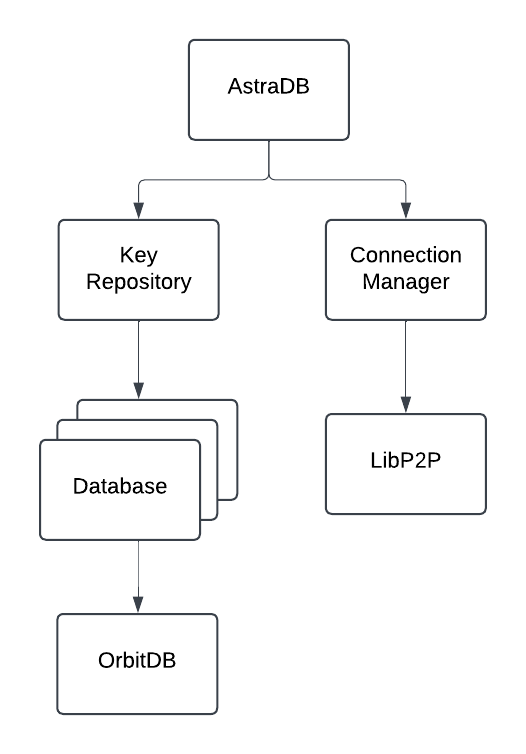
\includegraphics[width=0.5\linewidth]{img/solucion-ipfs/astradb-arquitectura.png}
\caption{Arquitectura de AstraDB.}
\label{fig:astradb-arquitectura}
\end{figure}

\paragraph{Key Repository}

El \textit{Key Repository} es el módulo encargado de la gestión integral de los datos dentro de la infraestructura. Su función principal consiste en mantener el registro de todas las claves existentes, así como efectuar las modificaciones necesarias sobre ellas.

Al iniciarse, este componente crea la base de datos central a partir del nombre recibido como parámetro y procede a sincronizarla con los colaboradores disponibles. Si no se logra establecer conexión con ningún colaborador, se asume que se trata de una base de datos nueva, y el módulo continúa su funcionamiento en modo autónomo.

En nodos configurados como colaboradores, al recibir actualizaciones sobre nuevas claves desde la base de datos central, el \textit{Key Repository} abre y almacena localmente la base de datos correspondiente a cada clave. Este proceso garantiza la persistencia de las claves y permite que otros usuarios accedan a ellas mediante sincronización.

Todas las bases de datos gestionadas por este módulo —tanto la central como las asociadas a cada clave— están representadas mediante una abstracción denominada \textit{Database}, la cual encapsula toda la interacción con OrbitDB.

Durante la inicialización, se define si la base debe sincronizarse o no. En caso afirmativo, el sistema espera conectarse con algún colaborador para obtener todas las actualizaciones disponibles. Una vez sincronizada, la base de datos queda habilitada para su uso, incluyendo la incorporación de nuevo contenido y la recuperación completa del mismo.

Además, toda actualización recibida en una base de datos gestionada por este módulo genera automáticamente un evento que puede ser escuchado por otros componentes del sistema. Esto permite implementar funcionalidades reactivas, como interfaces en tiempo real o disparadores personalizados, facilitando la integración de lógica adicional basada en los cambios del estado distribuido.

\paragraph{Connection Manager}

El \textit{Connection Manager} se encarga del manejo de conexiones entre nodos, incluyendo la búsqueda y establecimiento de conexiones con colaboradores que proveen la base de datos, así como la publicación del nodo como proveedor cuando este actúa como colaborador.

Al iniciarse, el módulo construye el \textbf{CID} (Content Identifier) correspondiente a la base de datos central. Para ello, utiliza \textbf{Helia} \cite{helia}, la implementación de IPFS en JavaScript, para calcular el identificador a partir del nombre recibido. Este CID es común a todas las instancias de AstraDB que utilizan dicho nombre, y permite que los nodos se identifiquen y sincronicen de forma coherente.

Luego, se inicializan tres servicios que operan concurrentemente durante la ejecución del sistema: \textit{SearchForProviders}, \textit{ProvideDB} y \textit{ReconnectToProviders}.

El servicio \textit{SearchForProviders} realiza búsquedas continuas de nuevos proveedores de la base de datos utilizando la DHT (Distributed Hash Table) de IPFS mediante \textbf{LibP2P} \cite{libp2p}. Cuando encuentra uno, intenta establecer conexión para iniciar la sincronización.

El servicio \textit{ProvideDB}, activo únicamente en nodos colaboradores, anuncia en la DHT que el nodo puede proveer la base de datos, facilitando su descubrimiento por parte de otros.

Finalmente, \textit{ReconnectToProviders} mantiene un listado de proveedores previamente conectados y realiza intentos periódicos de reconexión, asegurando la continuidad en caso de fallos temporales.

Estos servicios permiten que los nodos se descubran entre sí, compartan información de manera descentralizada y mantengan la red resiliente ante desconexiones o caídas parciales.

\paragraph{Implementación en los casos de uso}

La arquitectura y los mecanismos de AstraDB fueron puestos a prueba en dos casos de uso representativos: el repositorio de conocimiento y el mensajero en tiempo real.

En el caso del repositorio de conocimiento, las claves representaron los artículos de la wiki, mientras que los valores correspondieron a las modificaciones realizadas sobre cada artículo. De esta forma, fue posible reconstruir el estado actual de un artículo a partir de toda su historia de cambios almacenada.

Para el mensajero en tiempo real, cada clave representó un chat específico y los valores fueron los mensajes enviados en dicho chat. El sistema permitió el inicio de sesión de usuarios mediante la provisión de una clave privada, y habilitó la escucha en tiempo real de las actualizaciones en un chat determinado, garantizando así la recepción inmediata de nuevos mensajes.

Ambos casos de uso lograron, en su implementación, abstraerse del manejo directo del ecosistema subyacente —como IPFS, OrbitDB y LibP2P— gracias a los mecanismos provistos por AstraDB. Esta capa de abstracción permitió que los desarrollos se concentraran exclusivamente en la lógica específica de cada aplicación, sin necesidad de centrarse en detalles propios de la infraestructura distribuida.

Como resultado, no solo se cumplió con los requisitos funcionales de ambos casos, sino que se sentaron las bases para extender el sistema a nuevos escenarios. Siempre que las entidades de un caso de uso puedan representarse mediante claves y su evolución como una secuencia de eventos, AstraDB proporciona un entorno sólido y reutilizable para construir aplicaciones distribuidas de forma simple y modular.


\subsubsection{Colaboración}

Se creó una herramienta para facilitar la colaboración a nuestra wiki. El nodo es capaz de fijar los contenidos de Astraweb, nuestro front-end, y también mantener todas las bases de datos utilizadas por Astrawiki y Astrachat en la capa de aplicación. Para lograr esto, se diseñó un sistema con cuatro contenedores, cada uno asignado a uno de los tres casos de uso.

Para el pinning del sitio web en si, se utilizó el contenedor de IPFS Cluster con la instrucción de colaborar con el clúster dado por parámetro. Este parámetro es la dirección IPFS del archivo \texttt{service.json} que identifica a un clúster. Además, IPFS Cluster requiere de un contenedor de Kubo para manejar el manejo de archivos en la red de IPFS.

Para Astrawiki, se hizo uso del contenedor ofrecido por Astrawiki CLI, front-end que se verá más adelante. Con este contenedor, se puede actuar como colaborador fácilmente sin necesidad de interactuar con él.

Por último, Astrachat se levanta con un simple proyecto de Node que crea un nodo colaborativo y lo ejecuta en segundo plano.

\begin{figure}[H]
    \centering
    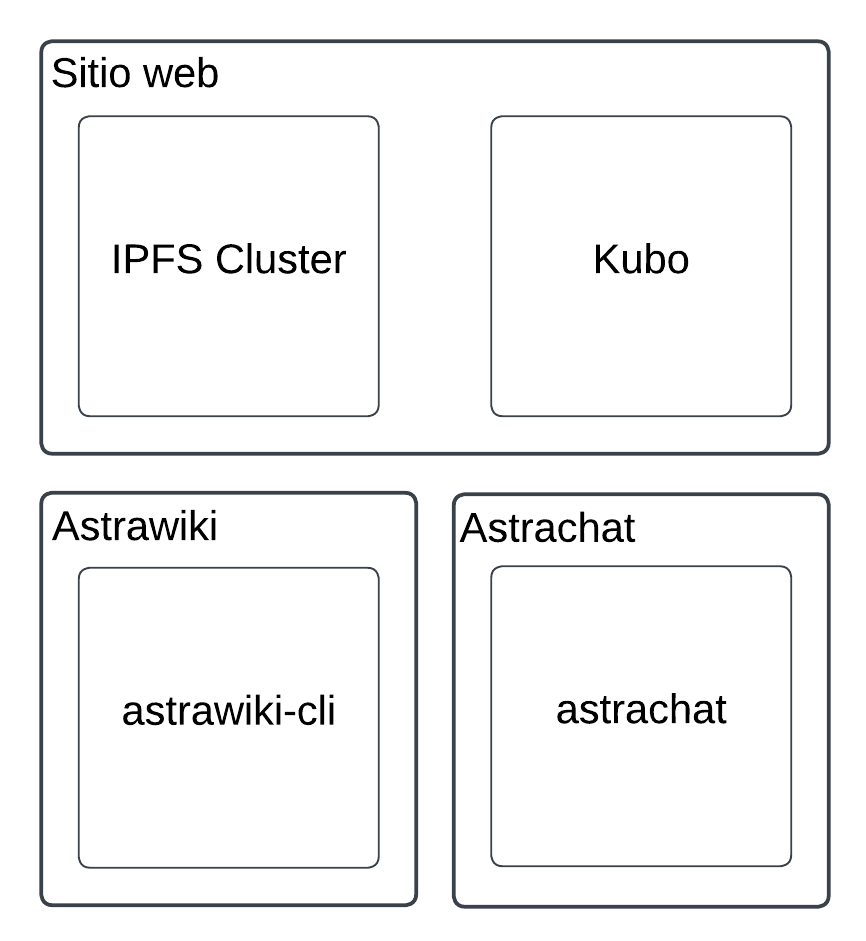
\includegraphics[width=0.5\linewidth]{img/solucion-ipfs/collaborator-arch.png}
    \caption{Arquitectura general del nodo colaborador}
    \label{fig:collaborator-architecture}
\end{figure}

Cada uno de estos casos se puede seleccionar o deseleccionar desde un archivo de configuración \texttt{.env}, para que el usuario pueda elegir en que parte del proyecto contribuir. El resultado es una herramienta que, si bien fue diseñada para Astraweb, puede utilizarse para cualquier tipo de front-end que utilice Astrawiki y/o Astrachat.
\subsection{Blockchain}

Para el ecosistema de blockchain se decidió utilizar la red de Ethereum \cite{wood2014ethereum}, al ser una blockchain popular y muy utilizada para el desarrollo de aplicaciones descentralizadas nos permite demostrar y comparar los casos de uso contra nuestra solución en IPFS.

\subsubsection{Swarm}

Existen varias soluciones de almacenamiento descentralizado dentro del ecosistema blockchain, en este caso, para el desarrollo del sitio web estático optamos por Swarm al estar basado en una \textit{sidechain} de Ethereum.

\paragraph{Feed} El contenido que se publica en Swarm tiene asociado un CID, esto lo hace inmutable. Para permitir cambios manteniendo la inmutabilidad del contenido en Swarm existen los \textit{feeds} que funcionan de manera similar a los nombres de IPNS en IPFS. Es un puntero, con CID fijo, a un archivo. Esto permite actualizar el archivo al que apunta un \textit{feed} manteniendo un punto de entrada fijo al sitio web.

\paragraph{Postage stamps} Esta es la forma de pagar por el uso del almacenamiento en la red de Swarm. Posee un \textit{time-to-live} (TTL) que es calculado en base a los valores de \textit{depth} y \textit{amount} indicados al momento de la creación del \textit{stamp} \cite{swarm-postage-stamps}.

\paragraph{Despliegue} Para el despliegue del \textit{front-end} es necesario primero comprar un \textit{postage stamp} con la moneda BZZ y luego con la herramienta \texttt{swarm-cli} \cite{swarm-cli} se publica el sitio web indicando el \textit{feed} correspondiente. Durante el desarrollo encontramos que no existe un \textit{gateway} público que apunte a la \textit{testnet} de Sepolia y nos permita probar el despliegue sin necesidad de utilizar dinero real. Es por esto que se levantó un nodo de Swarm configurado para que apunte a la \textit{testnet} de Sepolia y un \textit{gateway} que utilice este nodo mediante la herramienta \texttt{gateway-proxy} \cite{gateway-proxy} que provee el equipo de Swarm.

\subsubsection{Ethereum}

Para los casos de uso del repositorio de conocimiento y el mensajero en tiempo real necesitamos una herramienta que funcione de manera \textit{read-write} y como Swarm solamente se encarga de archivos estáticos buscamos alguna alternativa dentro del ecosistema blockchain. Para esto terminamos usando Ethereum.

\begin{figure}[H]
    \centering
    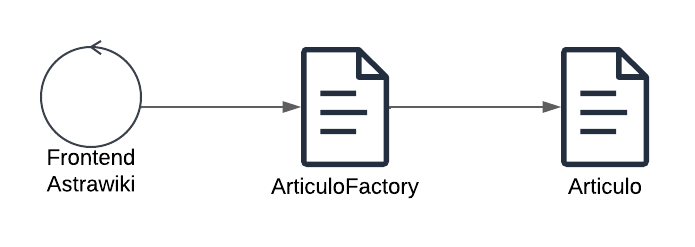
\includegraphics[width=0.5\linewidth]{img/astrawiki-articulo-factory.png}
    \caption{\textit{Smart contracts} que intervienen en el repositorio de conocimiento}
    \label{fig:aw-eth-articulo-factory}
\end{figure}

Ambos casos de uso resultaron muy similares en su resolución, haciendo uso del patrón de diseño \textit{Factory}. Existe un \textit{smart contract Factory} que crea otros \textit{smart contracts} (Artículo o Chat, según el caso de uso).

\begin{figure}[H]
    \centering
    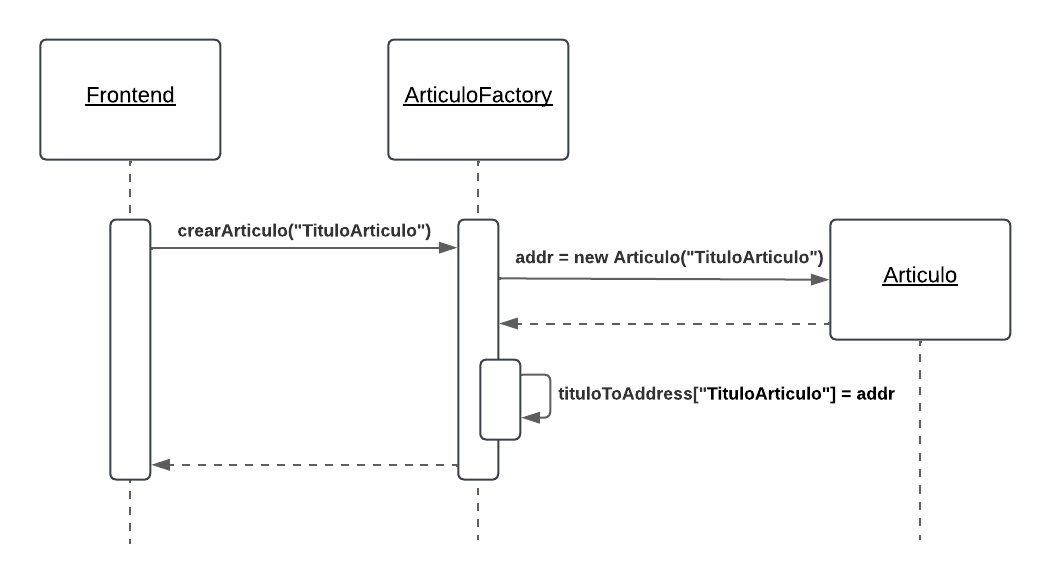
\includegraphics[width=0.75\linewidth]{img/ds-aw-eth-crear-articulo.png}
    \caption{Creación de un artículo}
    \label{fig:ds-aw-eth-crear-articulo}
\end{figure}

De esta manera el \textit{Factory} tiene un \textit{mapping} con todos los artículos creados y las direcciones correspondientes para accederlos. Si se quisiera acceder a un Artículo en particular primero se tiene que consultar al \textit{Factory} para obtener la dirección del mismo y, como cada artículo es un \textit{smart contract} en sí mismo, se puede consultar o modificar su contenido directamente interactuando con el Artículo en particular como se puede ver en la Figura \ref{fig:ds-aw-eth-obtener-contenido-articulo}.

\begin{figure}[H]
    \centering
    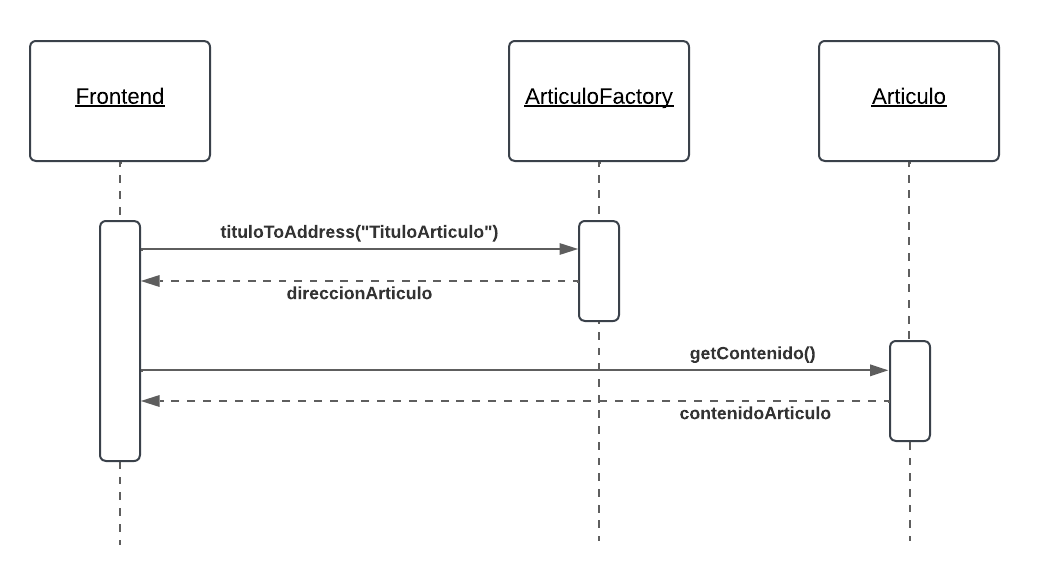
\includegraphics[width=0.75\linewidth]{img/ds-aw-eth-obtener-contenido-articulo.png}
    \caption{Obtención del contenido de un artículo}
    \label{fig:ds-aw-eth-obtener-contenido-articulo}
\end{figure}

La principal diferencia entre el repositorio de conocimiento y el mensajero en tiempo real está en que los mensajes del mensajero tienen que ser vistos por los demás usuarios que participan de la conversación en el momento que se envían. Esto no es estrictamente necesario en el repositorio de conocimiento pero sí lo es en el mensajero.

Para afrontar este requisito se utilizaron los eventos de Solidity (el lenguaje de programación en el que se desarrollan los \textit{smart contract} de Ethereum). Funciona de la siguiente manera, al momento de enviar un mensaje se emite un evento. Este evento se recibe en un \textit{listener} que fue previamente inicializado al instante previo de haber obtenido el Chat en el \textit{front-end}. Al recibir este evento el \textit{front-end} puede actualizar la pantalla mostrando el mensaje nuevo sin necesidad de obtener todos los mensajes.

% TODO: insertar gráfico del flujo de un evento al enviar un mensaje 

Por otro lado, para el mensajero en tiempo real necesitamos una manera de identificar a cada usuario. Para esto se hizo uso de las \textit{wallets}. Cada usuario se identifica utilizando su \textit{wallet}, que tiene una clave pública, que pasa a ser el identificador del usuario, y una clave privada la cuál es necesaria para firmar transacciones en nombre del usuario, que en nuestro caso funciona a modo de contraseña. Además, para que la lectura de las conversaciones sean más usables, se agregó la posibilidad de generar un nombre de usuario asociado al identificador del mismo. A este nombre de usuario lo llamamos alias y es único para todos los Chats asociados a un mismo \textit{ChatFactory}. Una vez el usuario se conecta con su \textit{wallet}, puede elegir un alias y cambiarlo cuando desee siempre y cuando no exista actualmente algún otro usuario con ese mismo alias.

Finalmente, nos queda la funcionalidad de que un usuario pueda responder a otro mensaje. Primero necesitamos una manera de identificar a cada mensaje de manera unívoca. El identificador de cada mensaje se genera \textit{hasheando el timestamp} del bloque, el identificador del emisor y la cantidad de mensajes en el chat en el momento que se envía. Luego, cuando se responde a otro mensaje se almacena el identificador del mensaje al que se está respondiendo (el mensaje padre) dentro de la estructura del mensaje que se está enviando. Todo esto se resuelve dentro del \textit{smart contract} del Chat correspondiente.

\subsection{Hyphanet}

Hyphanet \cite{hyphanet} es una plataforma peer-to-peer para publicar y comunicar, resistente a la censura y respetuosa de la privacidad.

Originalmente conocido como Freenet y creado como un trabajo profesional de fin de carrera por Ian Clarke, Hyphanet es una plataforma de software libre que permite compartir archivos, navegar y publicar sitios de forma anónima. Es descentralizado para hacerlo menos vulnerable a ataques, y de ser usado sólo con personas de confianza lo hace difícil de detectar.

\paragraph{Aplicaciones comunitarias}

La plataforma se basa en conexiones por nodos que gestionan la información que hay en la red. Estos nodos pueden conectarse a una red abierta llamada \textit{Opennet} en la cual las conexiones se harán con nodos de cualquier persona de cualquier parte del mundo. Por otro lado es posible configurar el nodo para que se conecte sólo con aquellas personas que uno conozca, creando así una red ''privada'' (o \textit{darknet}) en la que sólo personas de confianza puedan conectarse.

El contenido que se publica en los nodos permanece de forma encriptada y repartido en varias partes por distintos nodos. Siempre que un archivo sea solicitado el mismo será cacheado en los distintos nodos que lo soliciten.

No es posible ''borrar'' un archivo como tampoco es posible guardarlo a voluntad. Si un archivo no es suficientemente solicitado eventualmente no se puede recuperar más. Los nodos tampoco pueden elegir qué contenido (partes de un archivo) guardar o no ya que los mismos están encriptados. Si un archivo es subido por un nodo que no está disponible en este momento el archivo no se pierde porque ya fue distribuido por los demás nodos que estaban conectados a él.

% Para acceder a un archivo es necesario conectarse a la red e ingresar el hash correspondiente.

\subsubsection{Plugins}

Es posible crear aplicaciones de comunicación con los llamados \textit{plugins}. Estos \textit{plugins} deben ser hechos en el lenguaje Java (o al menos el \texttt{main} debe estarlo) por decisión de diseño (alegando que Java es ''más seguro''). No están aislados del sistema \textit{host} por lo que pueden acceder a toda la información que quieran. Se deben compilar y proveer el \texttt{.jar} correspondiente y cada usuario que quiera utilizarlo debe instalarlo en su respectivo nodo.

Entre los plugins más usados en el ecosistema podemos nombrar:

\subparagraph{WebOfTrust}\cite{hyphanet-web-of-trust}
Se autodenomina un spam filter pudiendo puntuar (\textit{trust values}) a cada usuario de forma que los que tienen puntaje muy bajo son catalogados como spammers y cualquier contenido que los involucre será filtrado.

\subparagraph{Sone}\cite{hyphanter-sone}
Red social similar a Facebook en el que se pueden subir imágenes, comentar, conectarse con otras personas. Usa WebOfTrust para identificar a cada usuario.

\subparagraph{Freemail}\cite{hyphanet-freemail}
Un servicio de email dentro de Hyphanet que también depende de WebOfTrust.

\subparagraph{Freetalk}\cite{hyphanet-freetalk}
Sistema de foro.

No hay una receta para implementar estos plugins ya que la guía que existe está incompleta y hace años que no se actualiza (lo mismo pasa con los plugins en sí, llevan años sin actualizarse).

La documentación brilla por su ausencia y cada plugin hace uso de la librería de \textit{Freenet} de una forma distinta lo cual hace difícil saber cuál es la forma correcta (de haberla) para crear un plugin desde cero.

Toda información que deba guardarse se debe hacer en una base de datos local administrada por el plugin (ya sea usando un archivo o una librería como podría ser \textit{sqlite}\cite{sqlite}) ya que no existe una base de datos distribuida en el ecosistema que lo facilite. Esto hace que cada nodo tenga la información sólo de aquellos nodos con los que interactúa, mientras más lo haga más datos va a tener que persistir. Además es necesario que el plugin tenga forma de garantizar la integridad de los datos sino podrían ser fácilmente manipulados por algún nodo generando inconsistencias para la aplicación (que a su vez debería poder manejar).

\subsubsection{Sitio web estático}

Hyphanet posee un software propio para poder agregar sitios llamado \textit{jSite}\cite{hyphanet-jsite}. Con el mismo, basta con seguir las instrucciones en la \href{https://www.hyphanet.org/pages/documentation.html}{documentación oficial}. Una vez finalizada la creación del sitio, el programa devolverá un \textit{hash} el cual será necesario para poder acceder al sitio.


\paragraph{Caso de uso}

Se logró levantar un sitio web estático que sólo contenía un HTML con un ''Hello World'' utilizando \textit{jSite}\cite{hyphanet-jsite} en el ecosistema.

\subsubsection{Otros casos de uso}

Debido a la escasa documentación y falta de estándares para desarrollar aplicaciones en el ecosistema, no se prosiguió con los demás casos de uso y se optó por investigar el ecosistema \textit{Freenet}.


\subsection{Freenet}

\textit{Freenet}\cite{freenet} es una red peer-to-peer para servicios descentralizados, sin censura, en donde los usuarios tengan el control del contenido.

Creado por Ian Clarke, el mismo creador de \textit{Hyphanet}\cite{hyphanet}, es una plataforma nueva que busca ser una computadora descentralizada en reemplazo de servidores centralizados. Está hecha en Rust y utiliza WebAssembly para ejecutar las aplicaciones.

Siguiendo las bases de Hyphanet, y a diferencia de IPFS, Freenet busca ser una \textit{computadora distribuida} donde cada peer es capaz de ejecutar código que contenga estado el cual tendrá eventual consistencia con los demás peers. Parecido a su antecesor, un contrato puede cachearse en varios peers si este es lo suficientemente popular y dejará de cachearse si deja de serlo.

\subsubsection{Arquitectura}

\paragraph{Key-value}

Freenet es un \textit{global key-value store} que se basa en la idea del \textit{small-world routing}\cite{freenet-small-world-routing} para la descentralización y escalabilidad. Las \textit{keys} son código WebAssembly en dónde se especifican:

\begin{itemize}
    \item Qué valores están permitidos en la \textit{key}.
    \item Bajo qué circunstancias el valor puede ser modificado.
    \item Cómo se puede sincronizar el valor eficientemente entre los \textit{peers} de la red.
\end{itemize}

\paragraph{Contracts}

La base de la comunicación de las aplicaciones distribuidas son los \textit{contracts}. Estos \textit{contracts} son código Rust compilado a WebAssembly donde una clase debe cumplir con la interfaz del contrato (\texttt{ContractInterface}). Este es encargado de mantener la consistencia del estado de la aplicación en los distintos \textit{peers}. Está pensado para que la actualización sea eficiente de modo que los \textit{contracts} se actualizan en base a las diferencias.

\paragraph{Contracts vs Smart Contracts}

Los \textit{contracts} de Freenet poseen ciertas similitudes y diferencias con los \textit{smart contracts} de Blockhain.

\setlength\tabcolsep{1pt}
\begin{table}[H]
    \centering
    \begin{tabular}{|m{21em}|m{10em}|m{10em}|}
        \hline
         & \textbf{Contracts (Freenet)} & \textbf{Smart Contracts (Blockchain)} \\
        \hline
        \textbf{¿Descentralizado?} & Si & Si \\
        \hline
        \textbf{¿Mantiene estado?} & Si & Si \\
        \hline
        \textbf{¿Puede ejecutar código arbitratiamente?} & Si (limitación local) & Si (limitación global) \\
        \hline
        \textbf{¿Se distribuye el estado entre distintas instancias?} & Si & No \\
        \hline
        \textbf{¿Pago?} & No & Si \\
        \hline
    \end{tabular}
    \caption{Comparativa entre Contracts de Freenet y Smart Contracts de Blockchain}
    \label{tab:contracts-vs-smart-contracts}
\end{table}

\paragraph{Comunicación}

Al momento de probar el ecosistema, una aplicación podía comunicarse con un contrato a través de un \textit{web socket}. De esta forma se busca mantener el estado actualizado en la aplicación local ante un eventual cambio hecho por otro \textit{peer}.

\subsubsection{Diferencias con Hyphanet}

\paragraph{Funcionalidad} Hyphanet es un disco duro descentralizado mientras que Freenet busca ser una computadora descentralizada.

\paragraph{Interacción en tiempo real} Freenet permite a los usuarios subscribirse a los datos y ser notificado inmediatamente ante algún cambio del mismo. Esencial para aplicaciones de chat o interacción en tiempo real.

\paragraph{Lenguaje de programación} Hyphanet fue desarrollado en Java. Freenet está implementado en Rust haciéndolo más eficiente y pudiéndose integrar mejor a los distintos sistemas operativos (Windows, Mac, Android, etc).

\paragraph{Transparencia} Freenet está pensado como un posible reemplazo a World Wide Web.

\paragraph{Anonimato} La versión anterior fue diseñada con foco en el anonimato. La nueva versión no ofrece esta opción \textit{out of the box} sin embargo es posible crear un sistema por encima que provea cierta anonimidad.
\subsection{Front-end}

% TODO: Mostrar un diagrama de cómo todos los paquetes de bitxenia se utilizan e interactuan entre sí para que el front-end los termine usando. 

Como prueba de la versatilidad de los ecosistemas, y aprovechando la creación de paquetes, se desarrollaron diferentes front-ends para las aplicaciones realizadas.

\paragraph{Astraweb}

Es el principal front-end, y acumula todos los casos de uso creados en una única aplicación web, demostrando la capacidad de utilizar estas herramientas en conjunto, en un entorno web, y de manera intercambiable. Se le permite al usuario escoger el ecosistema al que se desea conectar, pudiendo intercambiar ecosistemas libremente, a forma de comparar y evaluar la funcionalidad desarrollada en este proyecto.

Representa un repositorio de conocimiento, con discusiones en cada articulo, lo que se asemeja a repositorios como Wikipedia. Además, se alojan en las redes descentralizadas evaluadas, tanto en IPFS como en Swarm, accesibles desde el navegador.

\subparagraph{Funcionalidad}

Desde la página principal es posible seleccionar entre tres ecosistemas distintos:

\begin{itemize}
    \item Example Server
    \item IPFS
    \item Blockchain
\end{itemize}

Una vez seleccionado el ecosistema se puede acceder a la barra de búsqueda para buscar el artículo deseado o bien se puede crear un artículo.

En la creación de un artículo \ref{fig:astraweb-create-article}, es posible darle un nombre y una descripción la cual puede ser escrita en Markdown para darle estilo. Una vez dentro de un artículo \ref{fig:astraweb-article-page}, a la derecha se puede acceder al historial de versiones (donde se puede visualizar una versión específica del artículo), editar el artículo (sólo en contenido puede ser modificado) y también al chat del artículo.

Cada artículo posee un chat en tiempo real \ref{fig:astraweb-chat} que actúa como discusión para la mejora o modificación del mismo. Dentro del chat es posible enviar mensajes y responder a mensajes anteriores desde un alias configurado por el usuario. Para mantener la identidad dentro de los chats, se puede ingresar con la misma identificación.

\begin{figure}[H]
    \centering
    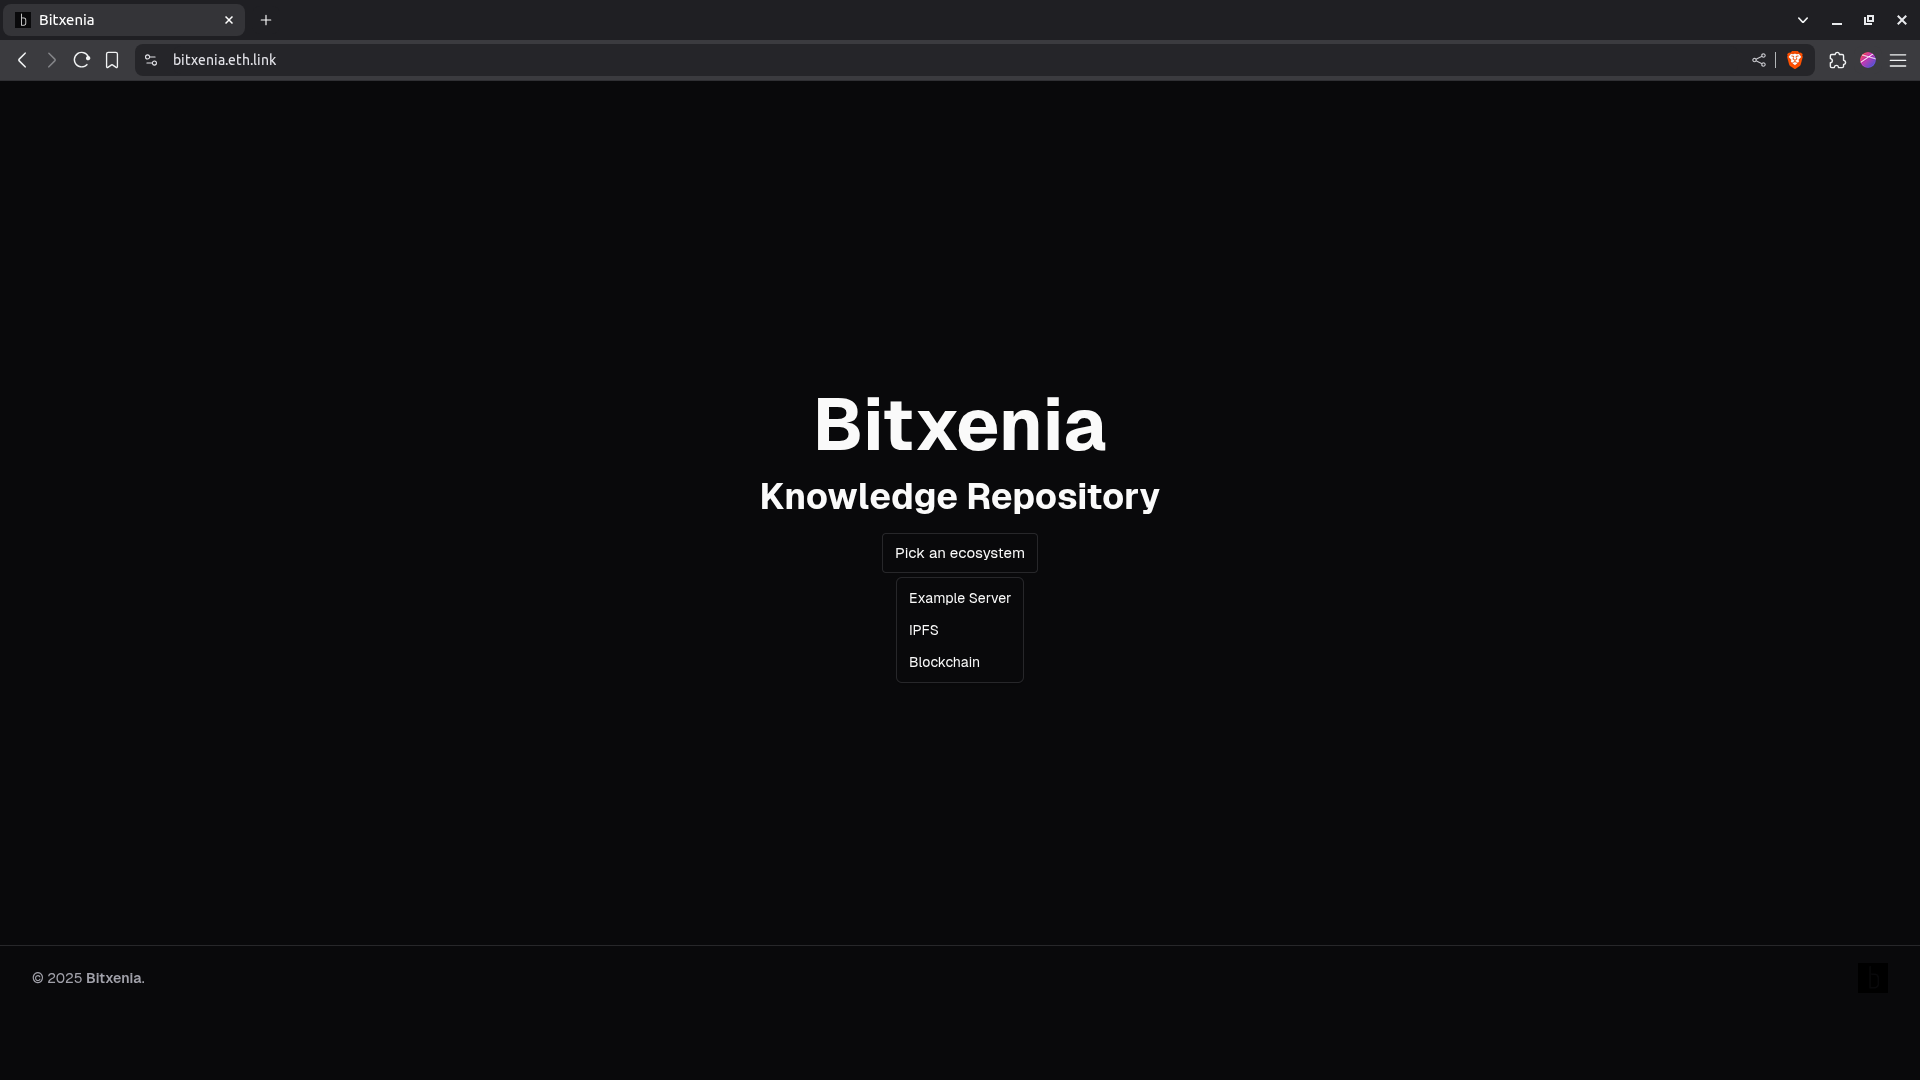
\includegraphics[width=1\linewidth]{img/frontends/astraweb-main-page.png}
    \caption{Página principal de Astraweb}
    \label{fig:astraweb-main-page}
\end{figure}

\begin{figure}[H]
    \centering
    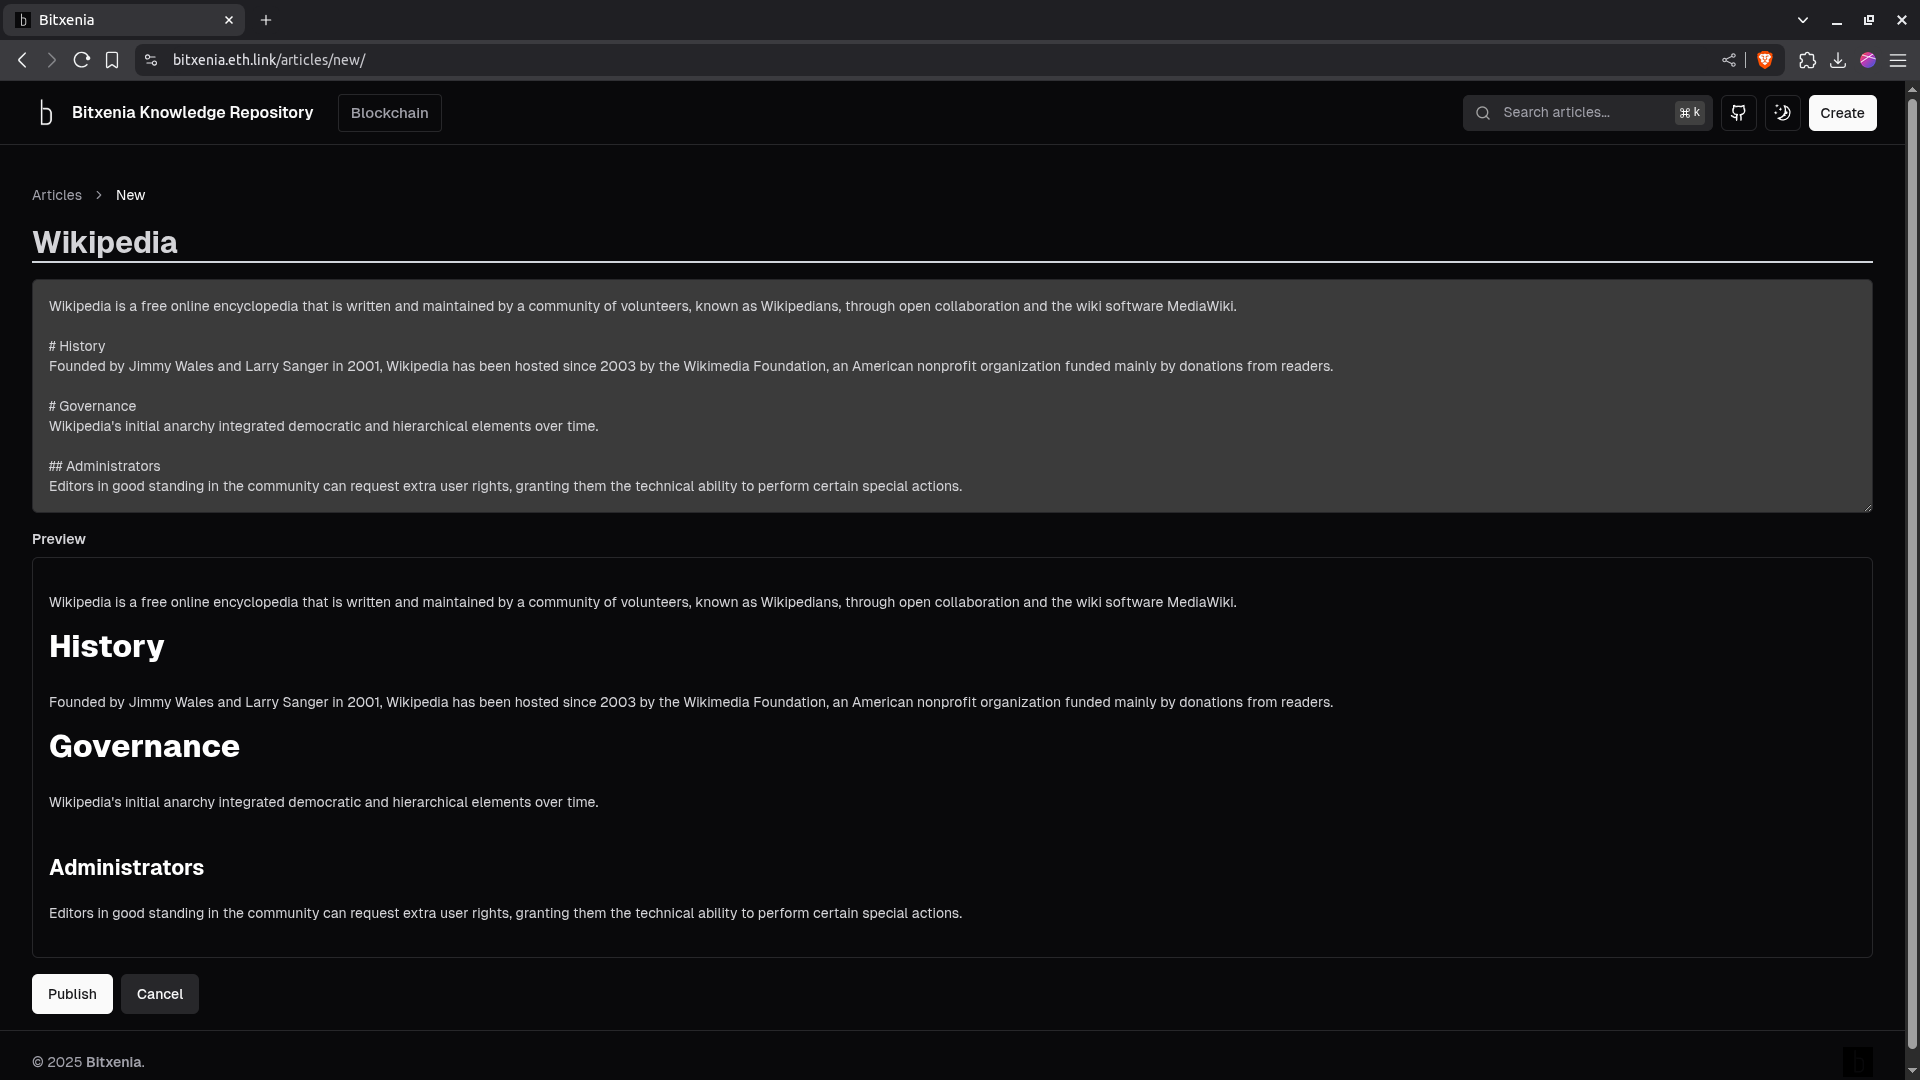
\includegraphics[width=1\linewidth]{img/frontends/create-article.png}
    \caption{Creación de un artículo}
    \label{fig:astraweb-create-article}
\end{figure}

\begin{figure}[H]
    \centering
    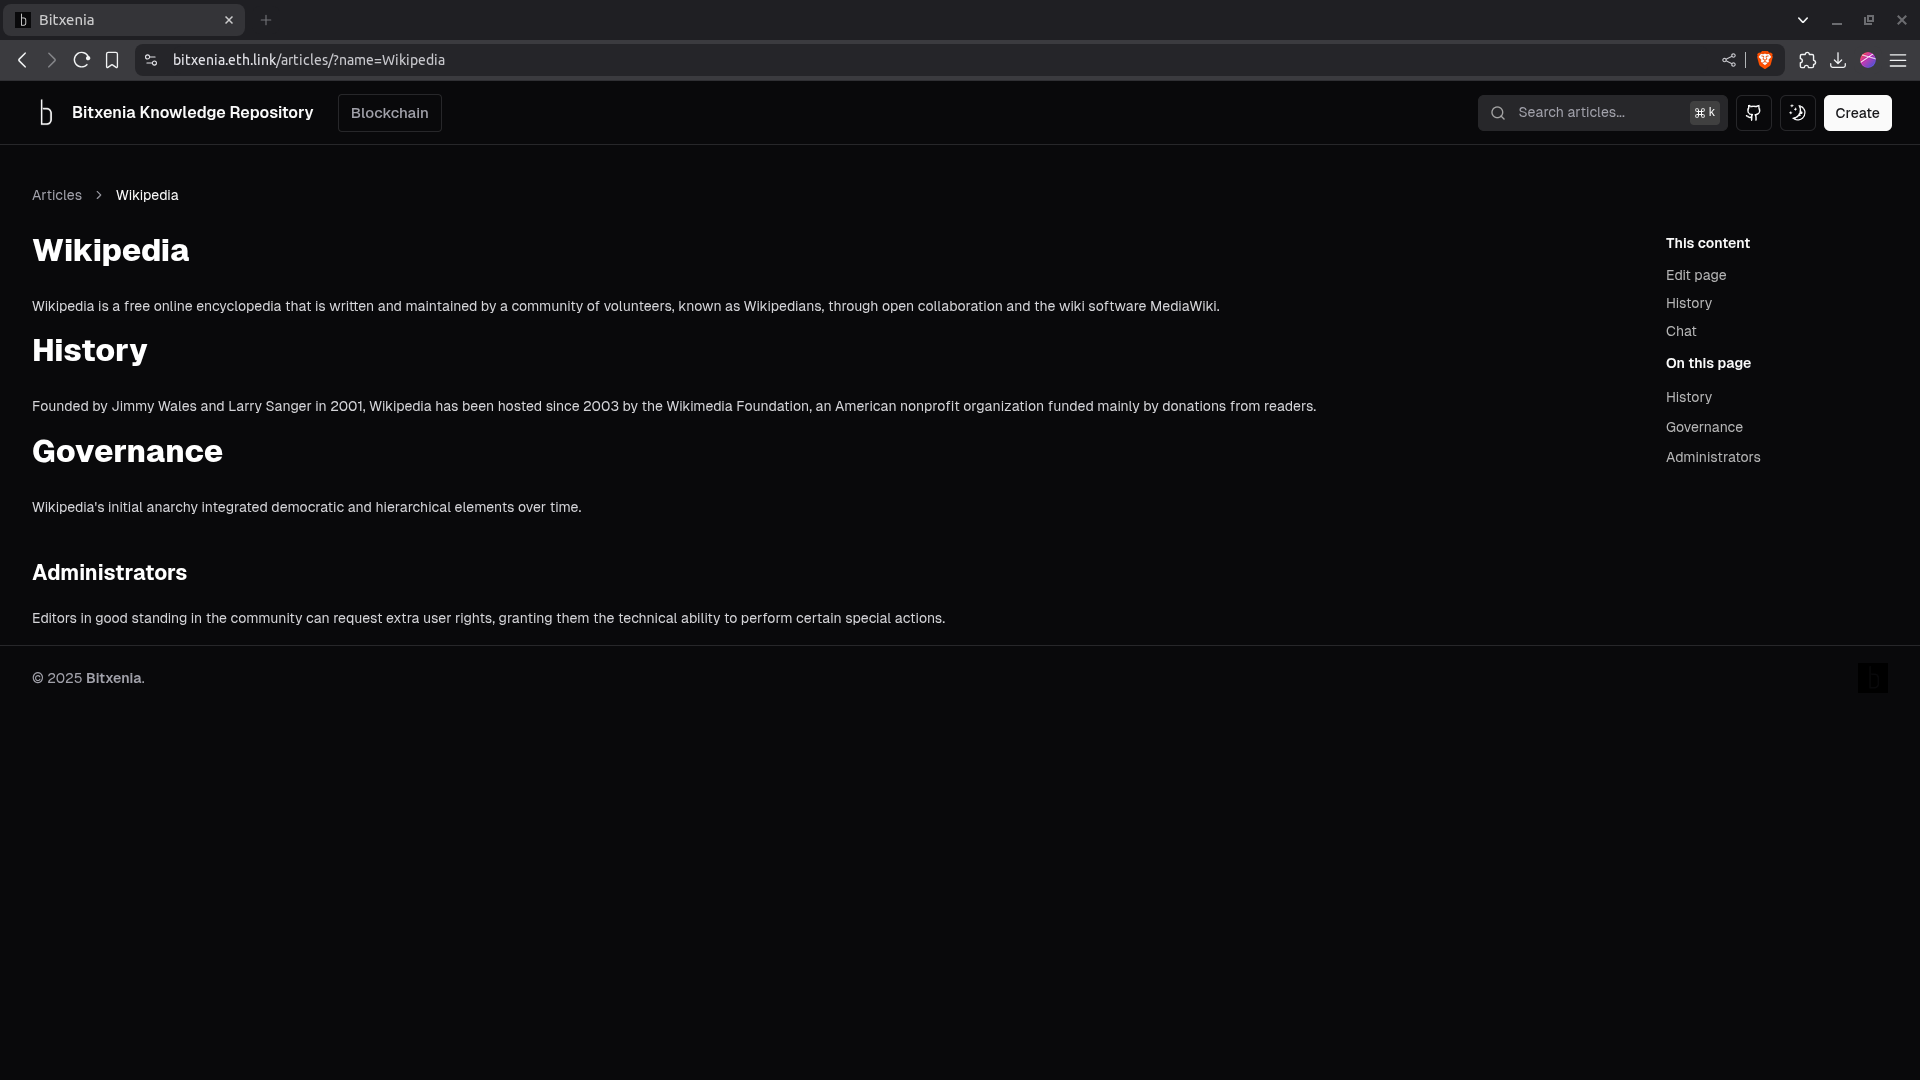
\includegraphics[width=1\linewidth]{img/frontends/article-page.png}
    \caption{Página de un artículo}
    \label{fig:astraweb-article-page}
\end{figure}

\begin{figure}[H]
    \centering
    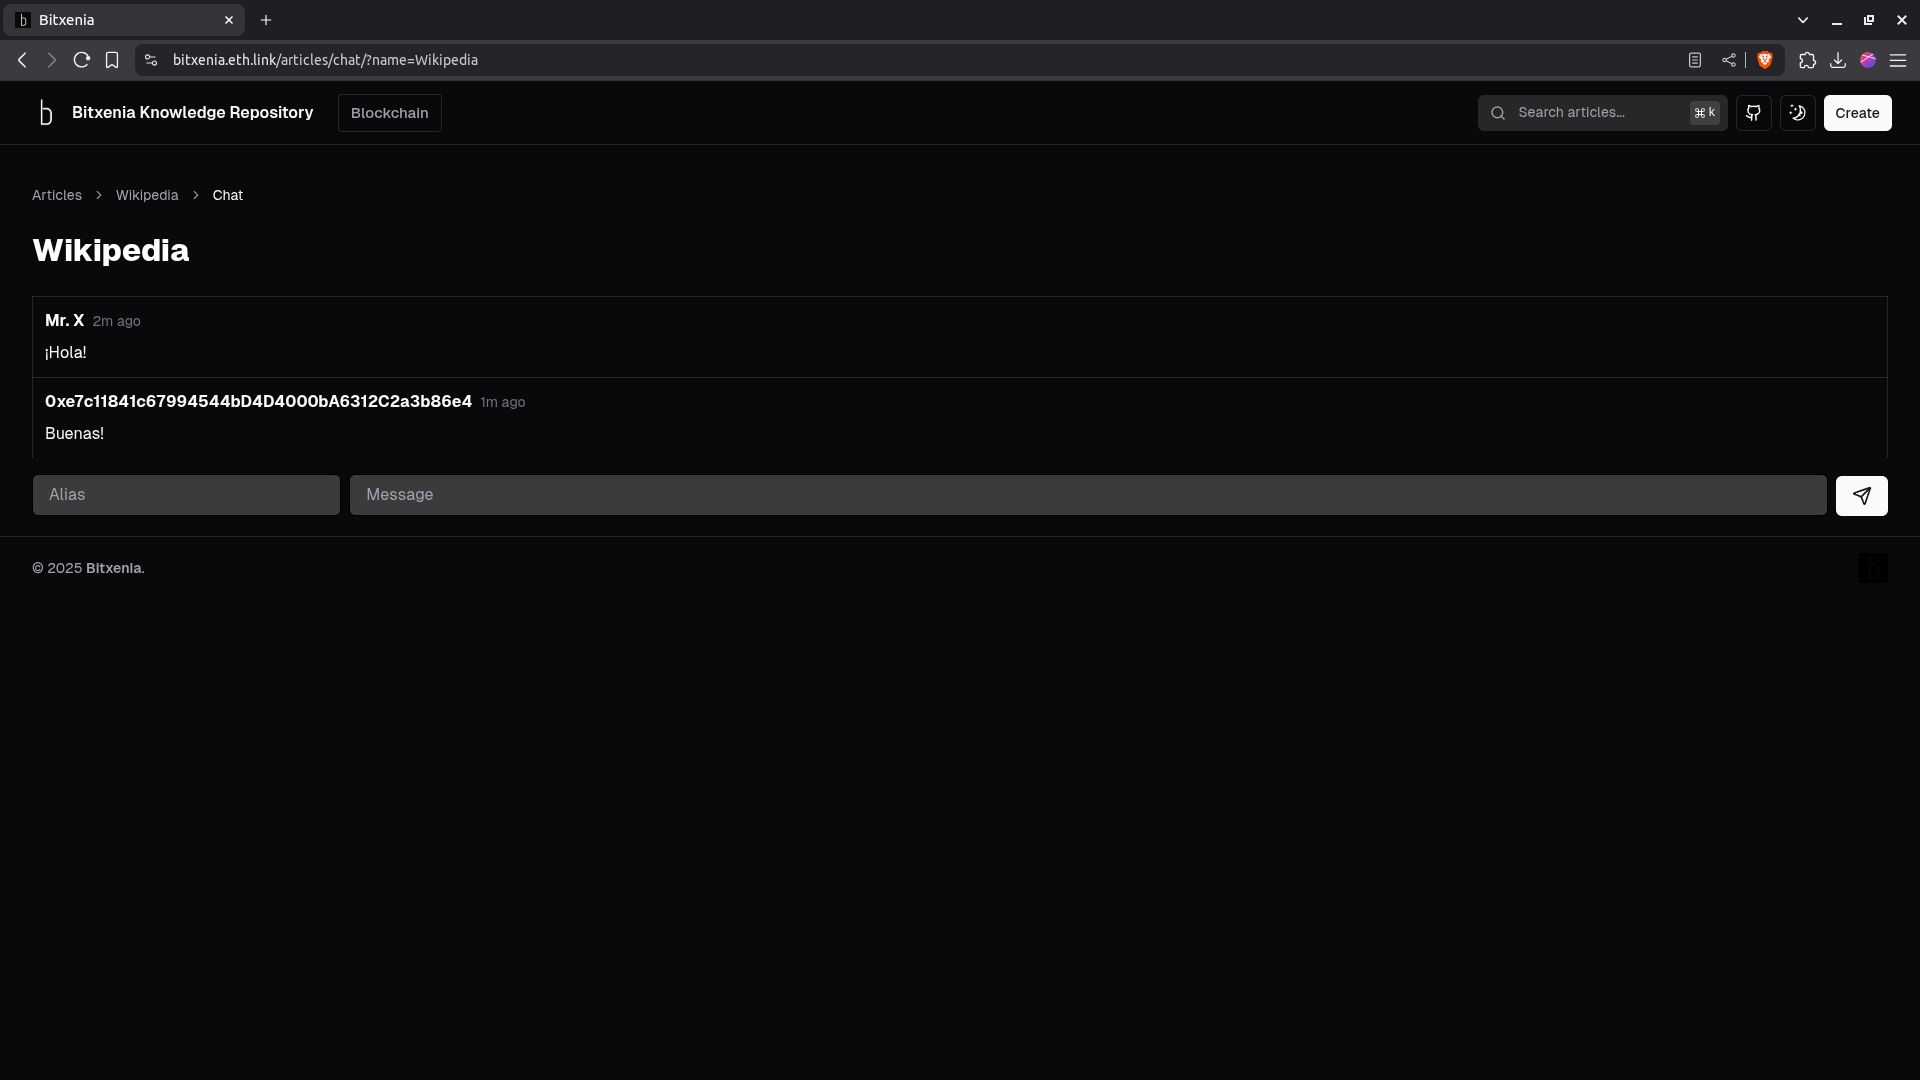
\includegraphics[width=1\linewidth]{img/frontends/astraweb-chat.png}
    \caption{Chat de un artículo}
    \label{fig:astraweb-chat}
\end{figure}

\subparagraph{Tecnología} Se utilizó \texttt{React} \cite{react} y \texttt{Next.js} \cite{next} como \textit{frameworks} para la creación de la aplicación web, basándonos en una plantilla llamada \texttt{rubix-documents} \cite{rubix}. El código fue escrito en \texttt{Typescript}.

\subparagraph{Servidor ejemplo} Se desarrolló una solución centralizada como tercer ecosistema para este frontend, con dos propósitos:
\begin{enumerate}
    \item Paralelizar el desarrollo del front-end y los distintos paquetes de cada ecosistema. Debido a que se definió una interfaz común tanto para el repositorio de conocimiento como para el mensajero en tiempo real, se logró avanzar con el front-end haciendo pruebas manuales con este servidor.
    \item Comparar las implementaciones descentralizadas contra un enfoque centralizado.
    % TODO: esto habría que sacarlo?
\end{enumerate}
El servidor fue creado en \texttt{Node.js} con \texttt{Express.js} como framework para interactuar con \textit{requests} de HTTP.

\subparagraph{Limitaciones} Debido a la falta de un servidor tradicional para ofrecer el contenido, el uso de \textit{Server Components} o componentes de servidor \cite{server-components} no era posible. Esto implicó modificar ampliamente la plantilla utilizada para descartar este tipo de componentes en favor de aquellos que pueden ser compilados y luego utilizados por el cliente sin interacción con un servidor.

\paragraph{Astrawiki CLI}

Front-end de terminal, desarrollado para el caso de uso del repositorio de conocimiento y para el ecosistema de IPFS en específico. Cuenta con todas las funcionalidades del repositorio de conocimiento, como crear, editar y ver artículos, consultar versiones pasadas, e incluso colaborar, lo cual se verá en el apartado de IPFS. Además, cuenta con un contenedor \texttt{Docker} publicado, con el fin de fácilmente iniciar un nodo sin necesitar una instalación de \texttt{Node} y demás dependencias. Funciona como un \texttt{daemon} \cite{daemon}, es decir, se inicia y funciona en segundo plano hasta que se indique lo contrario.

Su propósito es, por un lado demostrar la versatilidad del modelo de paquetes utilizado para crear distintos front-ends. Y por otro lado, el contenedor es útil para el nodo colaborador desarrollado para IPFS visto previamente.

\subparagraph{Arquitectura} Se compone de un cliente, el cuál se inicia con cada comando (\texttt{start}, \texttt{add}, \texttt{get}, \texttt{edit}, \texttt{list}, etc.) y un servidor que se ejecuta por detrás, el cual inicia la instancia del repositorio de conocimiento de IPFS y utiliza su API cuando recibe \texttt{requests HTTP}.

\begin{figure}[H]
    \centering
    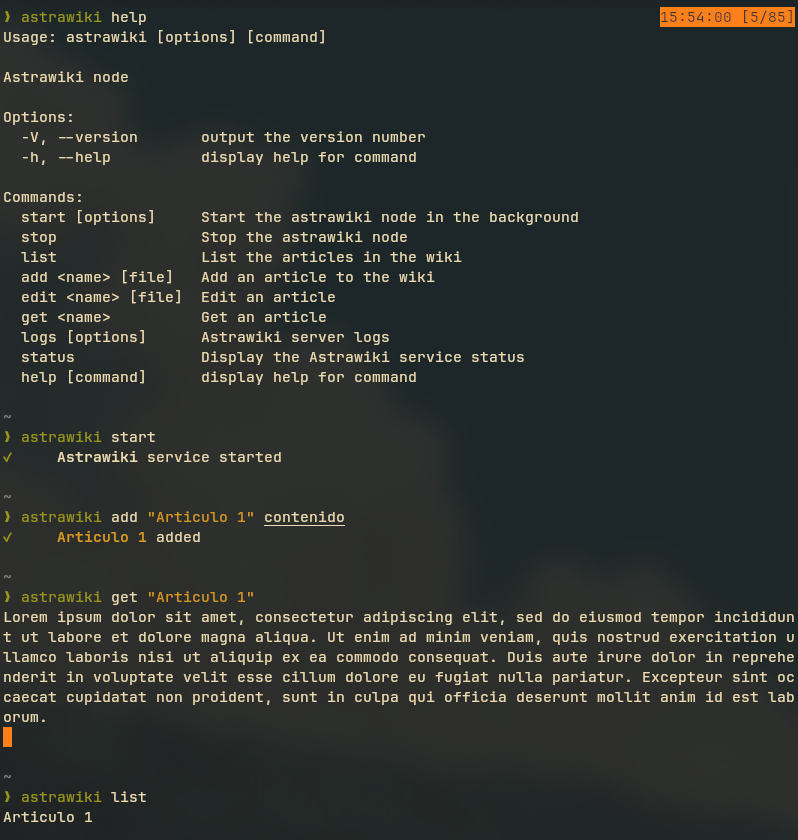
\includegraphics[width=0.7\linewidth]{img/astrawiki-cli.png}
    \caption{Ejemplo de uso de \texttt{astrawiki-cli}}
    \label{fig:astrawiki-cli}
\end{figure}

\paragraph{Astrachat CLI}

Frontend de terminal, desarrollado para el caso de uso de mensajero en tiempo real y para el ecosistema de Blockchain.

\subparagraph{Tecnología}

Se utilizó \texttt{React} \cite{react} y \texttt{Ink} \cite{ink} como \textit{frameworks} para crear la interfaz de este frontend.

\subparagraph{Funcionalidad}

Esta implementación permite crear un chat, unirse a un chat existente, enviar y leer los (últimos) mensajes. No provee de la opción de modificar el alias ni tampoco de responder a otro mensaje.

\begin{figure}[H]
    \centering
    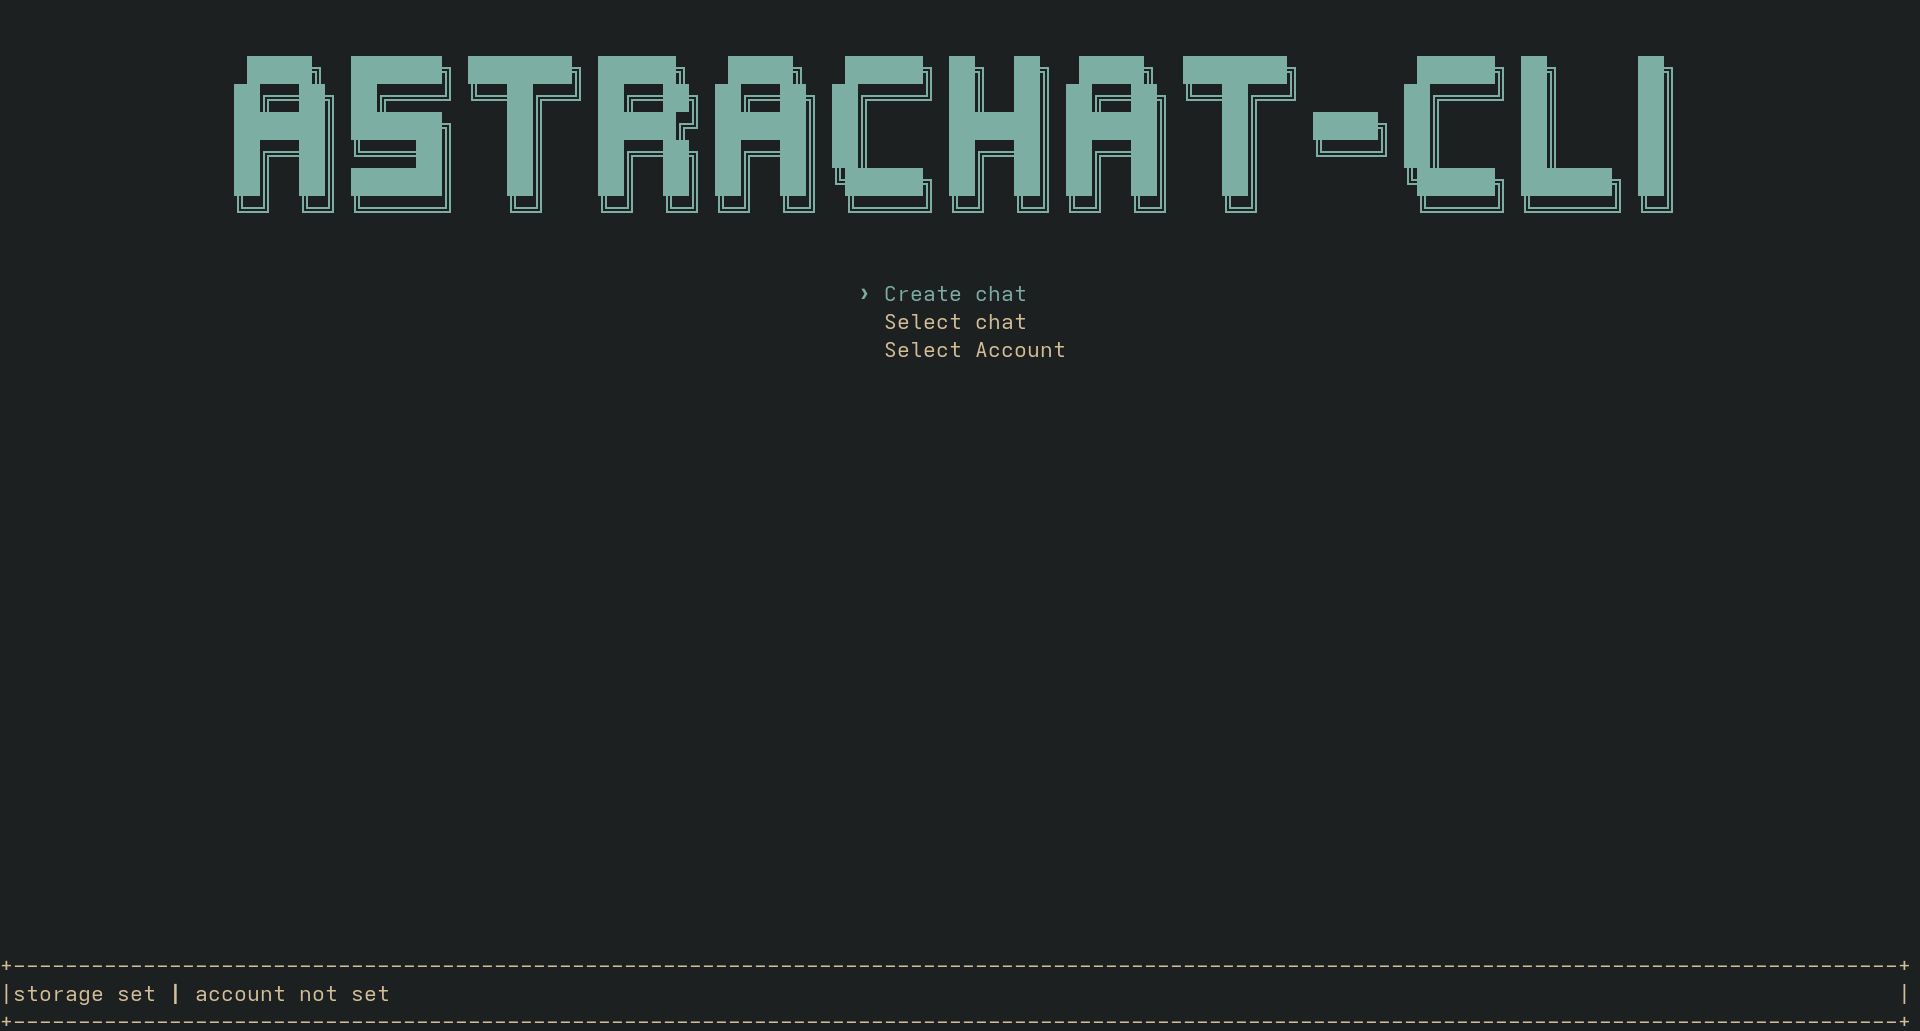
\includegraphics[width=1\linewidth]{img/astrachat-cli-main-page.png}
    \caption{Página principal de \texttt{astrachat-cli}}
    \label{fig:astrachat-cli-main-page}
\end{figure}

\subparagraph{Limitaciones}

Debido a que se ejecuta en la terminal no es posible hacer uso de una wallet como Metamask \cite{metamask} ya que la misma sólo funciona en web. Debido a esto, se \textit{hardcodearon} algunas de las wallets que provee Hardhat \cite{hardhat}.
